% $Id$
\documentclass[10pt]{article}
\usepackage{epsfig}
\usepackage{dcolumn}
\usepackage{alltt}

\def\numpackages{30}
\def\numpackageslesstwo{28}
\def\numlines{2 million}
\def\numlinesexact{nearly 2 million}
\def\numlinesncnbexact{about 1.4 million}

\newcommand{\pkg}[1]{\textsf{#1}}

\newcommand{\file}[1]{\texttt{#1}}

% the "fullpage" package does almost the same thing
% as the below lines-- it doesn't make things quite as
% tall or wide, but is generally what I use
% \usepackage{fullpage}
\marginparwidth 0pt
\oddsidemargin  0pt
\evensidemargin 0pt
\marginparsep 0pt
\topmargin   0pt
\headsep 0pt
\headheight 0pt
\textwidth   6.5 in
\textheight  9 in

\renewcommand{\floatpagefraction}{.8} %default .5
% Avoid putting all figures at end of text.
\renewcommand{\textfraction}{.1}  % .2 is the default
\renewcommand{\topfraction}{.9}   % .7 is the default

\begin{document}
% \bibliographystyle{plain}
\bibliographystyle{alpha}

\title{An Empirical Analysis of C Preprocessor Use}

\author{Michael D. Ernst%
  \and Greg J. Badros%
  \thanks{Supported by a National Science Foundation
    Graduate Fellowship. Any opinions, findings, conclusions, or
    recommendations expressed in this publication are those of the
    author, and do not necessarily reflect the views of the National
    Science Foundation.}
  \and David Notkin}

\date{% Technical Report UW-CSE-97-04-06 \\
Department of Computer Science and Engineering \\
University of Washington \\
Box 352350, Seattle, WA  98195-2350  USA \\
{\small \{{\tt mernst},{\tt gjb},{\tt notkin}\}{\tt @cs.washington.edu}} \\
2 November 1997}  

\maketitle

\begin{abstract}
  The C programming language is intimately connected to its macro
  preprocessor Cpp.  This relationship hinders tools built to engineer C
  programs, such as compilers, debuggers, call graph extractors, and
  translators.  Most tools make no attempt to analyze macro usage, but simply
  preprocess their input, which has a number of negative consequences.  In
  order to determine how the preprocessor is used in practice, and the
  feasibility of automatic analysis of preprocessor use, this paper
  analyzes {\numpackages} packages comprising {\numlines} lines of publicly
  available C code.  We determine the incidence of C preprocessor usage which
  is complex, potentially problematic, or inexpressible in in terms of
  other C or C++ language features.
[[We also came up with the list of things to investigate; and along the way
we taxonomized some stuff, which is also a contribution.]]

  We particularly note data that are
  material to the development of tools for C or C++, including translating
  from C to C++ to reduce preprocessor usage.  The results are of interest
  to language designers, tool writers, programmers, and software
  engineers.
[[ FIX: rewrite ]]
\end{abstract}

\bigskip

\section{Introduction}

The C programming language~\cite{ansi} is incomplete without its macro
preprocessor, Cpp~\cite[Ch.~3]{Harbison91}. By supplying such
facilities as file inclusion, definition of constants and macros, and
conditional compilation, Cpp can be used to define new syntax,
abbreviate repetitive or complicated constructs, or eliminate reliance
on a compiler implementation to inline functions, propagate symbolic
constants, eliminate dead code, and short-circuit constant tests.  Cpp
also permits system dependences to be made explicit and tested,
resulting in a clearer separation of concerns.  In addition, Cpp
permits a single source to contain multiple different dialects of C; a
frequent use is to support both K\&R-style and ANSI-style
declarations.  Indeed, one cannot write practical C programs without
these facilities.

While disciplined use of the preprocessor can reduce programmer effort
and improve portability, performance, or readability, Cpp is widely
viewed as a source of difficulty for understanding and transforming C
programs.  Because of Cpp's lack of structure\,---\,its inputs and
outputs are raw token streams\,---\,Cpp is very flexible, but lends
itself to arbitrary source code manipulations that complicate
understanding of the program by both software engineers and tools.  In
the worst case, the preprocessor makes merely determining the program
text as difficult as determining the output of an ordinary program.
The designer of C++, which shares C's preprocessor, also noted these
problems: ``Occasionally, even the most extreme uses of Cpp are
useful, but its facilities are so unstructured and intrusive that they
are a constant problem to programmers, maintainers, people porting
code, and tool builders.''~\cite[p.~424]{Stroustrup-DesignEvolution}

Tools\,---\,and, to a lesser degree, software engineers\,---\,have
three options for coping with Cpp.  They may ignore preprocessor
directives altogether, accept only post-processed code (usually by
running Cpp on their input), or attempt to emulate the preprocessor.
Each approach has different strengths and weaknesses.

\begin{itemize}

\item Ignoring preprocessor directives is an option for approximate
tools (such as those based on lexical or approximate parsing
techniques).  However, if accurate information about function extents,
scope nesting, declared variables and functions, and other aspects of
a program are required, the preprocessor cannot be ignored.

\item Operating on post-processed code, the most common strategy, is
simple to implement, but then the tool's input differs from what the
programmer sees.  Even when line number mappings are maintained, other
information is lost in the mapping back to the original source code.
For instance, source-level debuggers have no symbolic names or types
for constants and functions introduced via {\tt \#define}, nor can
tools trace or set breakpoints in function macros, as they can for
ordinary functions (even those that have been
inlined~\cite{Zellweger83:TR}).  As another example, Siff and Reps
describe a technique that uses type inferencing to produce C++
function templates from C; however, the input is ``a C program
component that $\ldots$ has been preprocessed so that all include
files are incorporated and all macros
expanded~\cite[p.~145]{Siff-fse96}.''  Such preprocessing may limit
the readability and reusability of the resulting C++ templates.  As
yet another related example, call graph extractors generally work in
terms of the post-processed code, even when a human is the intended
consumer of the call graph~\cite{Murphy-icse18}.  Some tools even
leave the software engineer responsible for inferring the mapping
between the original and the post-processed source, which is an
undesirable and error-prone situation.

In addition, a tool that manipulates post-processed code cannot be run
on a non-syntactic program or one that will not preprocess on the
platform on which the tool is being run.  These constraints complicate
porting and maintenance, two of the situations in which program
understanding and transformation tools are most likely to be needed.
Additionally, a tool supplied with only one post-processed
instantiation of the source code cannot reason about the program as a
whole, only about that version that results from one particular set of
preprocessor variables.  For instance, a bug in one configuration may
not be discovered despite exhaustive testing of other configurations
that do not incorporate particular code or do not admit particular
execution paths.

\item The final option, emulating the preprocessor, is fraught with
difficulty.  Macro definitions consist of complete tokens but need not
be complete expressions or statements.  Conditional compilation and
alternative macro definitions lead to very different results from a
single original program text.  Preprocessing adds complexity to an
implementation, which must trade off performing preprocessing against
maintaining the code in close to its original form.  Extracting
structure from macro-obfuscated source is not a task for the
faint-hearted.  Despite these problems, in many situations only some
sort of preprocessing or Cpp analysis can produce useful answers.

\end{itemize}

While much has been written about Cpp's potential pitfalls, no
previous work has examined actual use of the C preprocessor to
determine whether it presents a practical or merely theoretical
obstacle to program understanding, analysis, and transformation.  This
paper fills that gap by examining CPP use in {\numpackages} programs
comprising {\numlines} lines of source code.

The focus of the analysis is a set of potential pitfalls that might,
if present in practice, complicate the life of software engineerers
and tool builders:
\begin{description}
\item[high total use]  heavy use of either macro substitution or
  conditional compilation can overwhelm a human or tool; particularly
  problematic are lines that depend on many macros or macros that control
  many lines
\item[complicated bodies]  a macro body need not expand to a complete
  C syntactic entity (like a statement or expression)
\item[extra-linguistic features]  a macro body may exploit features of
  the preprocessor not available in C, such as stringization, token
  pasting, or use of free variables
\item[multiple definitions]  uncertainty about the expansion of a macro
  prevents knowledge of the actual program text; even more problematically,
  two definitions of a macro may be incompatible, for instance if one is a
  statement and the other expands to an expression or type
\item[macro pitfalls]  macros introduce new varieties or programming
  errors, such as function-like macros that fail to swallow a following
  semicolon and macros that fail to parenthesize, or side-effect, uses of
  formal variables
\item[inconsistent usage]  a macro used both for conditional
  compilation and to expand code is harder to understand than one used just
  for one purpose or the other
\item[mixed tests]  a single Cpp conditional may test conceptually
  distinct, unrelated conditions, making it difficult to perceive the
  intention
\item[variation in use]  if there is no clear pattern of use, or
  commonly-repeated paradigms, then no obvious point of attack presents
  itself
  %% No pattern according to package size, relative or absolute Cpp use, etc.
\end{description}
We report in detail on each of these aspects of preprocessor use,
indicating which appear to be innocuous in practice (that is, the
problematic uses appear only infrequently) and which may prove problematic
for software engineers.  We also present new taxonomies of macro body
expansions, macro feature usage, macro pitfalls, and conditional
intentions.  These taxonomies improve on previous work by being more
detailed and more accurately reflecting actual use.

Overall, our analysis confirms that the C preprocessor is used in
exceptionally broad and diverse ways, complicating the development of
C programming support tools.  In terms of the complexity of
preprocessor usage, the results reported here contain both good news
and bad.  By far the largest number of macro definitions and uses are
relatively simple, of the variety that a programmer could understand
without undue effort (although perhaps requiring tedious work) or that
a relatively unsophisticated tool could understand (although in
practice very few even try).  Despite the preponderance of innocuous
macros, the preprocessor is so heavily used that the remaining ones
are numerically significant.  It is precisely these macros that are
mostly likely to cause difficulties, and there are enough of them to
be problematic in practice and to make the effort of understanding,
annotating, or eliminating them worthwhile.

Sections~\ref{sec:first-content-section}--\ref{sec:last-content-section}
present the bulk of these results.  Section~\ref{sec:methodology}
describes our experimental methodology.  Section~\ref{sec:conclusion}
discusses the relevance of the research, suggests techniques for
mitigating the negative impact of Cpp on program understanding, and
discusses avenues for future work, while section~\ref{sec:related}
discusses related work.
%  The remainder of this section [[does some stuff]].

%[[Point reader at conclusion/summary of results, at end of paper (and write
%that!).]]

% \subsection{Outline}
% 
% The remainder of this paper is organized as follows.
% 
% Section~\ref{sec:directives} reports the percentage of original C source
% code lines that are preprocessor directives, including a breakdown of the
% frequency of specific directives such as {\tt \#define}.  C programs
% commonly have preprocessor directives as over 10\% of their total lines,
% and over 20\% of the lines were directives in 3 of the {\numpackages}
% packages.
% 
% Section~\ref{sec:usage} reports how often each macro is defined and
% expanded.   Identifiers tend to be {\tt \#define}d relatively few times
% (96\% of macro identifiers had three or fewer definitions).  Many packages
% also have a significant number of macros that are never expanded, even
% disregarding system and library header files.
% 
% Section~\ref{sec:categorization} categorizes macro definitions according to
% their expansions; for example, macros may simply define a preprocessor
% symbol, define a literal, expand to a statement, etc.  We were particularly
% interested in determining the frequency of use of macros that are difficult
% to convert to other language features, such as those that string together
% characters as opposed to manipulating lexemes or syntactic units (less than
% one third of one percent of all macro definitions),
% those that expand to partial syntactic units such as unbalanced
% braces or partial declarations (half of one percent), and others not 
% directly expressible in the programming language (about four percent).
% 
% Section~\ref{sec:conclusion} discusses the relevance of the research,
% suggests techniques for mitigating the negative impact of Cpp on program
% understanding, and discusses avenues for future work, while
% section~\ref{sec:related} discusses related work.


%[[Does anyone care about this?
%Another niche already filled by our tool is that of a ``macro lint''
%program which warns of potentially dangerous (or non-standard) uses of Cpp.
%And, we wrote CPPP.]]


% In order to assess the practical difficulty of understanding uses of CPP
% (and the potential for replacement by other language constructs), 





%Overall, our analysis confirms that the C preprocessor is used in
%exceptionally broad and diverse ways, complicating the development of C
%programming support tools.  On the other hand, the analysis also convinces
%us that, by extending our analysis framework with some class type
%inferencing techniques (similar to those used for C to C++
%translation~\cite{Siff-fse96} and for program
%understanding~\cite{OCallahan-icse97}), we can take significant
%steps towards a tool that usefully converts a high percentage of Cpp code
%into C++ language features.  We are interested not in translations
%that merely allow a C program to be compiled by a C++ compiler (which is
%usually easy, by intentional design of C++) but those that take advantage
%of the added richness and benefits of C++ constructs.
%
%[[Inane, content-free.  Must die.]]
%In terms of the complexity of preprocessor usage, the results reported here
%contain both good news and bad.  By far
%the largest number of macro definitions and uses are relatively simple, of
%the variety that a programmer could understand without undue effort (although
%perhaps requiring tedious work) or that a relatively unsophisticated tool
%could understand (although in practice very few even try).  Despite the
%preponderance of innocuous macros, the preprocessor is so heavily used that
%the remaining ones are numerically significant.  It is precisely these
%macros that are mostly likely to cause difficulties, and there are enough
%of them to be problematic in practice and to make the effort of
%understanding, annotating, or eliminating them worthwhile.
%
%
%\subsection{Coping with Cpp}
%
%Tools\,---\,and, to a lesser degree, software engineers\,---\,have three
%options for coping with Cpp.    They may ignore preprocessor directives
%(including macro definitions) altogether, accept only post-processed code
%(usually by running Cpp on their input), or attempt to emulate the
%preprocessor.
%
%Ignoring preprocessor directives is an option for approximate tools, such
%as those based on lexical or approximate parsing techniques.  Accurate
%information about function extents, scopes, declared variables and
%functions, and other aspects of a program requires addressing the
%preprocessor.
%
%Operating on post-processed code, the most common strategy, is simple to
%implement, but then the tool's input differs from what the
%programmer sees.  Even when line number mappings are maintained, other
%information is lost in the mapping back to the original source code.
%For instance, source-level debuggers have no symbolic names or types
%for constants and functions introduced via {\tt \#define}, nor can tools
%trace or set breakpoints in function macros, as they can for ordinary
%functions (even those that have been inlined~\cite{Zellweger83:TR}).
%As another example, Siff
%and Reps describe a technique that uses type inference to produce
%C++ function templates from C; however, the input is ``a C program
%component that $\ldots$ has been preprocessed so that all include
%files are incorporated and all macros
%expanded~\cite[p.~145]{Siff-fse96}.''  Such preprocessing may limit
%the readability and reusability of the resulting C++ templates.  As
%yet another related example, call graph extractors generally work in
%terms of the post-processed code, even when a human is the intended
%consumer of the call graph~\cite{Murphy-icse18}.  Some tools even
%leave the software engineer responsible for inferring the mapping between the
%original and the post-processed source, which is an undesirable and
%error-prone situation.
%
%A tool that first preprocesses code, or takes already-preprocessed code as
%input, cannot be run on a non-syntactic program or one that will not
%preprocess on the platform on which the tool is being run.  These
%constraints complicate porting and maintenance, two of the situations in
%which program understanding and transformation tools are most likely to be
%needed.  Additionally, a tool supplied with only one post-processed
%instantiation of the source code cannot reason about the program as a
%whole, but only about that version that results from one particular set of
%preprocessor variables.  For instance, a bug in one configuration may not
%be discovered despite exhaustive testing of other configurations that do
%not incorporate particular code or do not admit particular execution paths.
%
%The third option, emulating the preprocessor, is fraught with difficulty.
%Macro definitions consist of complete tokens but need not be complete
%expressions or statements.  Conditional compilation and alternative macro
%definitions lead to very different results from a single original program
%text.  Preprocessing adds complexity to an implementation, which must trade
%off performing preprocessing against maintaining the code in close to its
%original form.  Extracting structure from macro-obfuscated source is not a
%task for the faint-hearted.  Despite these problems, in many situations
%only some sort of preprocessing or Cpp analysis can produce useful answers.
%
%All three approaches would be unnecessary if programs did not use
%preprocessor directives.  This is exactly what Stroustrup suggests:
%\begin{quote}
%  I'd like to see Cpp abolished.  However, the only realistic and
%  responsible way of doing that is first to make it redundant, then
%  encourage people to use the better alternatives, and {\em then\/}\,---\,years
%  later\,---\,banish Cpp into the program development environment with the
%  other extra-linguistic tools where it
%  belongs~\cite[p.~426]{Stroustrup-DesignEvolution}.
%\end{quote}
%C++ contains features\,---\,such as constant variables, inline functions,
%templates, and reference parameters\,---\,that obviate many uses of Cpp.
%Thus, translation to C++ is a path for partial elimination of Cpp.
%This study indicates the
%feasibility\,---\,and our framework for analyzing preprocessor usage
%provides a basis for the development\,---\,of an automatic translator with
%two attractive properties.  It would take as input C programs complete with
%preprocessor directives, and it would map many uses of directives into C++
%language features.  (It is not 
%practical to eliminate all uses of Cpp.  For example, C++ currently
%provides no replacement for the {\tt \#include} directive, or for
%stringization or pasting.  Macros that cannot be eliminated might be
%annotated with their types or 
%effects on parser or program state, so that even tools that do no Cpp
%analysis can operate correctly on such programs.)
%
%[[Where do these two points go?]]
%
%Another niche already filled by our tool is that of a ``macro lint''
%program which warns of potentially dangerous (or non-standard) uses of Cpp.
%
%And, we wrote CPPP.

%O'Callahan and Jackson also use type
%inference, although for program understanding rather than translation;
%they, too, apply their techniques to post-processed
%code~\cite{OCallahan-icse97}.


%\subsection{Cpp: not all bad}
%
%[[This section is out of place and horrible.  Where should the information
%go?]]
%
%Despite its evident shortcomings, Cpp is a useful and often necessary
%adjunct to C, for it provides capabilities unavailable in the language or
%its implementations.  Cpp permits definition of portable language
%extensions that can define new syntax, abbreviate repetitive or complicated
%constructs, or eliminate reliance on a compiler implementation to
%open-code (inline) functions, propagate symbolic constants, eliminate dead
%code, and short-circuit constant tests.  The latter guarantees are
%especially valuable for compilers that do a poor job optimizing or when the
%programmer wishes to override the compiler's heuristics.  Cpp also permits
%system dependences to be made explicit and tested, resulting in a clearer
%separation of concerns.  Finally, Cpp permits a single source to contain
%multiple different dialects of C; a frequent use is to support both
%K\&R-style and ANSI-style declarations.
%
%%% NEED A REFERENCE TO DEBUGGER HERE!
%%% also mention Emacs hide-ifdef mode
%
%Our long-term goal is not to take these useful features away from
%programmers, but to reduce Cpp use, making programs easier for humans to
%understand and tools to analyze.






\section{Methodology}
\label{sec:methodology}

We analyzed {\numpackages} publicly-available software packages which
represent a mix of application domains, authors, programming styles, and
sizes.  Some are interactive, while others are not, and some are graphical
while others are text-based, command-line applications.
Figure~\ref{fig:packages} describes the packages and lists their sizes in
terms of physical lines (newline characters) and non-comment, non-blank
(NCNB) lines.  The NCNB figure disregards lines consisting of only comments
or whitespace, as well as lines in a conditional that cannot evaluate to
true (such as {\tt \#if 0}, which is frequently used to comment out code).  The
remainder of our analysis uses the NCNB length, which more accurately
reflects the amount of source code.

\begin{figure}
\centering
{% ``\small'' here does have an effect, despite previous comment to the contrary
  \small
  \setlength{\tabcolsep}{.25em}
  \begin{tabular}{|l|r|r|r|r|l|}\hline
Package & Version & Physical lines & NCNB lines & Files & Description\\\hline\hline
bash & 1.14.7 & 67,604 & 46,110 & 151 & Command shell \\\hline
bc & 1.03 & 7,483 & 5,184 & 28 & Desktop calculator \\\hline
bison & 1.25 & 11,434 & 7,676 & 33 & Parser generator \\\hline
cvs & 1.9 & 79,670 & 53,431 & 208 & Revision control system \\\hline
dejagnu & 1.3 & 64,650 & 40,286 & 150 & Testing framework \\\hline
emacs & 19.34 & 206,309 & 134,251 & 445 & Text editor\\\hline
flex & 2.5.3 & 18,969 & 13,289 & 32 & Scanner generator \\\hline
fvwm & 2.0.43 & 55,584 & 42,498 & 151 & Window manager \\\hline
g77 & 0.5.18 & 133,366 & 98,980 & 232 & Fortran compiler \\\hline
gawk & 2.15.6 & 27,705 & 18,567 & 61 & GAWK interpreter \\\hline
gcc & 2.7.2.1 & 500,752 & 324,620 & 706 & C and C++ compiler\\\hline
genscript & 1.3.2a & 12,049 & 8,166 & 32 & Text-to-PostScript converter \\\hline
ghostview & 1.5 & 11,535 & 8,897 & 23 & PostScript previewer \\\hline
gnuchess & 4.0pl77 & 30,090 & 18,538 & 41 & Chess player \\\hline
gnuplot & 3.50.1.17 & 38,209 & 29,582 & 59 & Graph plotter \\\hline
groff & 1.10 & 68,872 & 60,054 & 162 & Text formatter \\\hline
gs & 262 & 77,695 & 56,378 & 309 & PostScript interpreter \\\hline
gzip & 1.2.4 & 9,067 & 5,774 & 34 & File compressor \\\hline
m4 & 1.4 & 16,778 & 10,327 & 28 & Macro expander \\\hline
mosaic & 2.6 & 126,026 & 79,753 & 289 & WWW browser\\\hline
perl & 5.003 & 66,856 & 57,450 & 88 & Perl interpreter \\\hline
plan & 1.5.3 & 23,826 & 18,870 & 68 & Schedule planner \\\hline
python & 1.4 & 82,466 & 62,137 & 221 & Python interpreter \\\hline
rasmol & 2.5 & 27,218 & 22,109 & 27 & Molecular visualization\\\hline
rcs & 5.7 & 17,979 & 11,843 & 28 & Revision control system \\\hline
remind & 3.00.15 & 18,222 & 13,130 & 41 & Schedule reminder \\\hline
workman & 1.3 & 13,419 & 9,653 & 24 & Audio CD player \\\hline
xfig & 3.1.4 & 53,244 & 42,020 & 120 & Drawing program \\\hline
zephyr & 2.0.4 & 42,665 & 29,118 & 242 & Notification system \\\hline
zsh & 3.0.1 & 46,197 & 35,377 & 43 & Command shell \\\hline
\hline
Total & & 1,955,939 & 1,364,068 & 4,076 & 30 packages\\\hline
\end{tabular}

%%% Local Variables: 
%%% mode: latex
%%% TeX-master: t
%%% End: 

}
\caption{Analyzed packages and their sizes.  NCNB lines are non-comment,
  non-blank lines.}
\label{fig:packages}
\end{figure}

Before performing our analysis, we ran {\tt configure} or the equivalent on
each package in order to prepare it for compilation.  This creates various
header files (such as \file{configure.h}).  Our analysis works in the
absence of this step, but warns about uses of never-defined macros and
under-reports some values related to those missing definitions.  We did
not, however, compile the packages; our analysis does not require that the
package be compilable (or even that the preprocessor be able to run on it).

We generated a list of all the C files in the package (both code and header
files).  In general, these have extensions like \file{.c}, \file{.h},
\file{.cc}, \file{.cpp}, \file{.hxx}, etc.  We removed files with such
extensions that don't actually contain valid C, and added others which were
{\tt \#included} by valid C files (some included files had extension
\file{.def}).

We analyzed all the C files in the package, as well as every file {\tt
\#include}d by any of those, primarily library header files.  We
took care to include as many libraries as possible so as not to overlook
those definitions.  However, the figures reported in this paper always omit
all macros defined only in libraries, as well as all macro uses in
libraries.  This prevents libraries from 
swamping the characteristics of the package code, which is our focus in
this study.  The programmer generally has no control over libraries and
their header files, and may not even know whether a library symbol is
defined as a macro or a true function or variable.  Finally, we assume that
library macros are carefully written to behave correctly and robustly
(sadly, we discovered this not to always be true in practice; an
analysis of library macros is outside the scope of this report).

Our analysis is a true whole-program analysis; rather than preprocessing the
code and examining just one configuration, we examine all possible code and
ignore no possible  conditional compilation conditions (though we do skip
over those which can be statically proven to be false).   As a result, this
analysis is more thoroughgoing than traditional ``whole-program'' analyses.

[[We merge different Cpp branches in the code wherever possible.  Discuss
this a bit.]]

We perform approximate parsing because the input is not a valid C program;
as a result, we miss some constructs, but we can cope with uncompilable C
and with partial constructs in conditional compilation branches.  Our tool
includes parsers for expressions, statements, and declarations.

We performed our analysis via a collection of Perk scripts, totaling
approximately 11,000 lines (7,000 NCNB lines).  The raw data, which
includes considerable data not reported here, and the programs used to
generate and manipulate them, are available from the authors.







\section{Occurrence of preprocessor directives}
\label{sec:directives}
\label{sec:first-content-section}

Figure~\ref{fig:directives-breakdown} shows how often preprocessor
directives appear in the programs we analyzed.  Each group of bars in the
figure represents the percentage of non-comment, non-blank (NCNB) lines
attributed to the specified category of directives, with each individual
bar showing the percentage for a specific package.  Conditional compilation
directives ({\tt \#if}, {\tt \#ifdef}, {\tt \#ifndef}, {\tt \#else}, {\tt
\#elif}, {\tt \#endif}) are grouped together.

\begin{figure}
\centerline{\epsfig{file=fig/directives-breakdown.eps,height=7.5in}}
\caption{Preprocessor directives as a fraction of non-comment,
  non-blank (NCNB) lines.}
\label{fig:directives-breakdown}
\end{figure}

The prevalence of preprocessor use makes understanding CPP constructs
crucial in any analysis of a program.  One in ten program lines is a
preprocessor directive rather than C code.  Across
packages, the percentage varies from less than 4\% to more than 22\%.
(These figures do not include the 28\% of lines which expand a macro or the
38\% of lines whose inclusion is controlled by {\tt \#if}; see
section~\ref{sec:dependence}.)

% \#if 46\%, \#define 35\%, \#include 13\%, \#undef 3\%, \#line 2\%

Conditional compilation directives account for just under half (46\%) of
the total directives in all packages, macro definitions comprise another
35\%, and file inclusion makes up most of the rest.  Packages are not very
uniform in their mix of preprocessor directives, however.  (If they were,
each group of bars in figure Figure~\ref{fig:directives-breakdown} would be
a scaled version of the top group.)  In particular, the prevalence of {\tt
\#include} is essentially independent of incidence of other directives.
The percentage of conditional directives varies from 16\% to 74\%, the
percentage of {\tt \#define} varies from 14\% to 52\%, and the percentage
of {\tt \#include}s varies from 4\% to 60\%.  This variation in usage
indicates that a tool for understanding Cpp cannot focus on just a subset
of directives.  


\subsection{{\tt \#line}, {\tt \#undef}, and other directives}

The definedness of a macro is often used as a boolean value.  However, {\tt
\#undef} is rarely used to set such macros to ``false''$\!$.  Most uses of
{\tt \#undef} immediately precede a definition of the just-undefined macro,
to avoid preprocessor warnings about incompatible macro redefinitions.

Every use of {\tt \#line} (in \pkg{bash}, \pkg{cvs}, \pkg{flex}, \pkg{fvwm},
\pkg{gawk}, \pkg{gcc}, \pkg{groff}, and \pkg{perl}) appears in lex or yacc
output that enables packages to build on systems lacking lex, yacc, or
their equivalents.  For instance, \pkg{flex} uses itself to parse its
input, but also includes an already-processed version of its input
specification (that is, C code corresponding to a {\tt .l} file) for
bootstrapping.

% , as are ``other'' directives (such as ).  
% as well as user-defined ones like {\tt \#module}

Rarely-appearing directives such as {\tt \#pragma}, {\tt \#assert}, and
{\tt \#ident}, and unrecognized directives, are omitted from
figure~\ref{fig:directives-breakdown}.  Among the packages we studied,
these directives account for .017\% of directives, or one in six thousand.
Their only significant user is \pkg{g77}, which contains 154 uses of {\tt
\#error} (representing 1.5\% of its preprocessor directives and 0.16\% of
its NCNB lines) to check for incompatible preprocessor flags.  We ignore
the null command (``{\tt \#}'' followed by only whitespace), which produces
no output.


\subsection{Packages with heavy preprocessor use}

The \pkg{gzip}, \pkg{remind}, and \pkg{bash} packages deserve
special attention for their heavy preprocessor usage\,---\,22\%, 21\%, and
16\%, respectively.

\pkg{gzip} {\tt \#define}s disproportionately many macros as literals and
uses them as arguments to system calls, enumerated values, directory
components, and more.  These macros act like {\tt const} variables and are
evidence of good programming style.  \pkg{gzip} also contains many
conditional compilation directives, since low-level file operations (such
as setting creation time and access control bits, accessing directories,
and so forth) are done differently on different systems.

\pkg{remind} supports speakers of multiple natural languages by using {\tt
\#define}d constants for basically all user output.  It also contains
disproportionately many conditional compilation directives; over half of
these test the definedness of \verb|HAVE_PROTO|, in order to provide both
K\&R and ANSI prototypes.

Like \pkg{gzip}, \pkg{bash} is portable across a large variety of
systems, but \pkg{bash} uses even more operating system services.
Ninety-seven percent of \pkg{bash}'s conditional compilation directives
test the definedness of a macro whose presence or absence is a boolean
flag indicating whether the current system supports a specific feature.
The presence or absence of a feature requires different (or sometimes
additional) system calls or other code.


\section{Macro definition bodies}
\label{sec:categorization}

This section examines features of macro definitions that may complicate
understanding the containing program.  We report how many macro definitions
expand to a partial or unidentifiable syntactic entity, take advantage of
special Cpp features that lie outside the programming language, or contain
other error-prone constructs.  We then turn to multiple definitions of a
particular macro name.  Multiple definitions can complicate understanding,
even if they do effectively the same thing.  We report on incidence of
redefinitions and of differing redefinitions, especially redefinitions with
incompatible bodies.

[[Punchline/summary goes here.]]



\subsection{Macro body categorization}

We categorized macro bodies into 28 categories, though for simplicity of
presentation, this paper coalesces these into ten higher-level categories.
We started with a set of categories that we expected to occur frequently
(similar to other macro
taxonomies~\cite{Stroustrup-DesignEvolution,Carroll95}), then iteratively
refined them to break up overbroad categories or add unforeseen ones.

Figure~\ref{fig:categorization} reports, for each package, how many
definitions create an expansion which falls in each category.  Macros which
act like C language constructs\,---\,such as variables or
functions\,---\,are easiest to understand and to translate into the
programming language, so there is reason to be optimistic for the 70\% of
macros whose bodies are expressions and the 6\% that are statements.  Other
macros, especially those which do not expand to a complete syntactic
construct, are more problematic.


The ten categories are as follows.  The examples are chosen for clarity
and brevity from the packages studied.

% Where does this go?
% There's no pattern, again.  (Nor is there a pattern by package size
% or by type of application.)

% The following isn't quite enough to get the columns lined up in this table.
% \newcolumntype{d}{D{.}{.}{2}}
% \begin{tabular}{|l|d|d|d|d|d|d|d|}\hline
\begin{figure}
% {\small
%   \setlength{\tabcolsep}{.25em}
%   \centerline{\begin{tabular}{|l|c|c|c|c|c|c|c|}\hline
Package & Null define & Literal & Expression & Statement & Stringization and pasting & Other syntatic macros & Failed classification\\\hline
Python & 176 & 510 & 865 & 50 & 5 & 62 & 21\\\hline
bash & 717 & 679 & 637 & 3 & 3 & 62 & 30\\\hline
bc & 4 & 36 & 37 & 2 & 0 & 9 & 1\\\hline
bison & 4 & 64 & 32 & 0 & 0 & 2 & 0\\\hline
cvs & 106 & 683 & 530 & 58 & 0 & 69 & 116\\\hline
flex & 32 & 224 & 87 & 19 & 0 & 36 & 2\\\hline
fvwm & 48 & 748 & 122 & 11 & 0 & 27 & 1\\\hline
gawk & 49 & 243 & 391 & 11 & 0 & 59 & 23\\\hline
genscript & 8 & 71 & 39 & 0 & 0 & 9 & 0\\\hline
gnuchess & 12 & 201 & 93 & 5 & 0 & 5 & 1\\\hline
gnuplot & 134 & 577 & 244 & 3 & 0 & 18 & 9\\\hline
groff & 18 & 607 & 148 & 11 & 1 & 36 & 98\\\hline
gzip & 110 & 229 & 130 & 25 & 0 & 21 & 4\\\hline
m4 & 36 & 83 & 272 & 26 & 0 & 62 & 1\\\hline
plan & 9 & 208 & 43 & 4 & 0 & 4 & 2\\\hline
rcs & 15 & 54 & 80 & 14 & 0 & 18 & 3\\\hline
remind & 11 & 744 & 108 & 65 & 0 & 18 & 2\\\hline
workman & 1 & 41 & 25 & 2 & 0 & 0 & 0\\\hline
xfig & 31 & 681 & 240 & 24 & 0 & 20 & 0\\\hline
zephyr & 80 & 451 & 255 & 28 & 0 & 27 & 2\\\hline
zsh & 31 & 520 & 267 & 20 & 0 & 40 & 5\\\hline
\hline
Total & 1632 & 7654 & 4645 & 381 & 9 & 604 & 321\\\hline
\end{tabular}}%
% }
\centerline{\epsfig{file=fig/def-categories.eps,height=6in}}
\caption{Categorization of macro definition bodies.  The legend numerically
  represents the information in the top row[[; the category names in the
  legend should be read across, by rows]].}
\label{fig:categorization}
\end{figure}


{
\label{sec:categorization-details}

\begin{description}
  \sloppy
  \emergencystretch=2em

%%  mcat_NULL: 5391
%%    100%  null_define (5391)
% @mcat_NULL = qw( catNULL_DEFINE );
\item[Null define]  The {\tt \#define} directive gives only an
  identifier name but no macro body, as in {\tt \#define
  \verb|HAVE_PROTO|}\@.  Such macros appear frequently in Cpp
directives (such as {\tt \#ifdef}), where they are used as boolean
variables by the preprocessor.  In code, they often represent optional
syntax.  For instance,
macro {\tt private} may expand either to {\tt static} or to nothing,
depending on whether a debugging mode is set.

%%  mcat_CONSTANT: 18971
%%    0.00%  constant (0)
%%    97%  literal (18426)
%%    2.9%  some_constant (545)
% @mcat_CONSTANT = qw( catCONSTANT catLITERAL catSOME_CONSTANT );
\item[Constant] The macro body is either a literal (97\% of this category)
  or an operator applied to constant values (3\% of this category).
  These macros act like {\tt const} variables. 
  For instance, {\tt \#define NULL 0}, {\tt \#define \verb|ARG_MAX|
  131072}, and {\tt \#define ETCHOSTS "/etc/hosts"} define literals, while
{\tt \#define \verb|RE_DUP_MAX| ((1<<15)-1)} and {\tt
\#define \verb|RED_COLS| (1 << \verb|RED_BITS|)} (where \verb|RED_BITS| is
a constant, possibly a literal) define constants.  This category includes
both macros whose value is invariant across all configurations of the
package and those which depend on other compile-time values.  

%%  mcat_NONCONSTANT_EXPRESSION: 13529
%%    100%  expression (13529)
% @mcat_NONCONSTANT_EXPRESSION = qw( catEXP );
\item[Expression]  The macro body is an expression, as in {\tt \#define
  sigmask(x) (1 << ((x)-1))} or {\tt \#define mtime mailfiles[i]->\verb|mod_time|}.
Such a macro acts like a function which returns a value (though the
macro need not take any arguments, so its uses may look syntactically
unlike function calls). 
The expression might have a single constant value everywhere (the usual
case for expression macros without arguments, most of which are classified
as constants, above) or might have a different value on each use (the usual
case for expression macros with arguments).

%%  mcat_STATEMENT: 2656
%%    47%  statement (1242)
%%    45%  semicolonless_statement (1197)
%%    1.5%  partial_statement (40)
%%    3.0%  statements (79)
%%    3.5%  semicolonless_statements (94)
%%    0.15%  partial_statements (4)
% @mcat_STATEMENT = qw( catSTATEMENT catSTATEMENT_SANS_SEMI catPARTIAL_STATEMENT
%                        catSTATEMENTS catSTATEMENTS_SANS_SEMI catPARTIAL_STATEMENTS );
% These aren't great examples (not from actual code); but so be it, as the
% actual examples are *very* long.
\item[Statement]\label{item:statement-category}
  The macro body is a complete statement such as
\begin{verbatim}
    #define L_ORDINAL_OVERRIDE plu = ".";
    #define FREE(x) if (x) {free(x); x=NULL;}
    #define SWALLOW_LINE(fp) { int c; while ((c = getc(fp)) != '\n' && c != EOF); }
\end{verbatim}
  Such a macro is like a function returning {\tt void}, except that uses
  should not be followed by a semicolon (see section~\ref{sec:lint}).
    
  To reduce the number of categories in this presentation, the statement
  category aggregates single statements (comprising 47\% of the category),
  statements missing their final semicolon (as in {\tt \#define QUIT if
  (\verb|interrupt_state|) \verb|throw_to_top_level|()}; these account
  for 45\%), multiple statements (3.0\%), multiple statements where the
  last one is missing its final semicolon (3.5\%), and partial statements
  (as in {\tt \#define ASSERT(p) if (!(p)) botch(\verb|__STRING|(p));
  else}; these are the final less than 2\% of the statement category).

%%  mcat_TYPE: 697
%%    82%  type (569)
%%    0.00%  partial_type (0)
%%    3.3%  declaration (23)
%%    15%  semicolonless_declaration (105)
% @mcat_TYPE = qw( catTYPE catPARTIAL_TYPE catDECLARATION catDECLARATION_SANS_SEMI);
% #my @mcat_DECLARATION = qw( catDECLARATION catDECLARATION_SANS_SEMI );
% #folded DECLARATION into the above, TYPE
% The DECLARATION ones are quite rare.
\item[Type] 
  These macros expand to a type or partial type (such as a storage class),
  or expand to a declaration (possibly missing its terminating semicolon).
  Examples include {\tt \#define \verb|__ptr_t|
  void~*}, {\tt \#define \verb|__INLINE| extern inline}, {\tt \#define
private static}, {\tt \#define \verb|FLOAT_ARG_TYPE| union
\verb|flt_or_int|}, and {\tt \#define CMPtype SItype}.  As a result, these
macros may be tricky to understand, and cannot be eliminated via
straightforward translation (though C++ templates may provide some hope).



%%  mcat_SYNTAX: 189
%%    18%  mismatched_entities (34)
%%    82%  punctuation (155)
% This includes ( catUNBALANCED catPUNCTUATION )
\item[Syntactic]  The macro body is either punctuation (82\% of this
  category; for example, {\tt \#define AND ;}) or contains unbalanced
  parentheses, braces, or brackets.  The latter are often used to create a
  block and perform actions that must occur at its beginning and end, as
  for \verb|BEGIN_GC_PROTECT| and \verb|END_GC_PROTECT|.
  Macros in this category are inexpressible in the underlying programming
  language, but depend on the preprocessor's manipulation of uninterpreted
  token streams; see also section~\ref{sec:extra-linguistic}.

%%  mcat_SYMBOL: 870
%%    1.7%  reserved_word (15)
%%    94%  function_name (820)
%%    4.0%  symbols (35)
%%  fudged to:
%%    1.8%  reserved_word (15)
%%    98%  function_name (820)

% @mcat_SYMBOL = qw( catRESERVED_WORD catFUNCTION_NAME catSYMBOLS);
\item[Symbol]
  The macro body is a single identifier that is either a function name
  (98\% of this category) or a reserved word (2\%, much of it uses of
  variable names such as {\tt new} which are reserved words in another
  C dialect).  A macro body which is a macro name inherits that macro's
  classification rather than appearing here.


%%  mcat_SYMBOL_UNKNOWN: 2765
%%    100%  unknown_symbol (2765)
% @mcat_SYMBOL_UNKNOWN = qw( catSYMBOL_UNKNOWN );
\item[Unknown symbol]
  The macro expands to a single symbol which is not defined in the package
  or in any library header files included by the package.  The symbol may
  be defined by compiler command arguments or may be used only inside an
  appropriate conditional compilation guard because it is only meaningful
  with a particular architecture, system, or library (for which we did not
  have header files available).
  
  Unknown symbols can also be variables or functions that we failed to
  parse.  Our approximate parser can succeed where an exact parse would not
  (as for unsyntactic code or entities interrupted by preprocessor
  directives), but sometimes fails to recognize declarations or
  definitions.


%%  mcat_NON_C_CODE: 639
%%    90%  command_line_arguments (574)
%%    10%  assembly_code (65)
% @mcat_NON_C_CODE = qw( catCOMMAND_LINE catASSEMBLY_CODE );
\item[Not C code]\label{page:not-c-code}
  The predominant use of such macros is for filenames and operating system
  command lines (together, 90\% of this category) and assembly code (the
  remaining 10\%).  The former usually appear in a file which is used by
  the preprocessor when run over both code and Makefiles.\footnote{Cpp's
    specification states that its input should be syntactic C code, so it
    can avoid performing replacements in comments and string constants.
    Cpp may not behave as expected when its input is not C, so it is good
    style to avoid such uses.  In practice, such uses have forced many C
    preprocessors to make fewer assumptions about their input than they
    otherwise might be able to.}  Our heuristics misclassify some such
  macros\,---\,after all, {\tt \#define \verb|SYSDEP_CFLAGS| -43 -w}
  creates a perfectly valid C expression.  (See the ``expression plus not C
  code'' line at 0.14\% in figure~\ref{fig:subset-categories}.)  The
  assembly code component includes only macros whose expansion is assembly
  code, not all expressions and statements that contain snippets of
  assembly code.

%%  mcat_FAILURE: 802
%%    0.00%  uncategorized (0)
%%    7.9%  being_categorized (63)
%%    10%  never_defined (82)
%%    78%  failed_categorization (628)
%%    3.6%  multiply_categorized (29)
% @mcat_FAILURE = qw( catNOT_YET catIN_PROCESS catNO_DEF catFAILURE catMULTIPLE );
\item[Failed classification]
  Our tool failed to categorize less than 2\% of the 46462 definitions, and
  8 of the {\numpackages} packages had no macro classification failures.
  No one variety of macro stands out among the failures, so a more complete
  categorization is unlikely to affect our conclusions.
  
  Some failures resulted from limitations of our parser, which does not
  handle pasting (defined in \section~\ref{def:pasting}), C++, or some
  non-portable C extensions.  Handling of partial entities is incomplete,
  so case labels, parts of structure declarations, and partial expressions
  are left unclassified.  Heuristics for recognizing operating system
  command lines or flags occasionally fail.  Additional failures result
  from macro bodies which cannot be unambiguously assigned to another
  category because their syntactic class depends on their
  arguments\,---\,such as {\tt \#define EXFUN(name, proto) name proto} and
  {\tt \#define
\verb|DO_OP|(OP,a,b) (a OP b)}.  Finally, macros in bodies were not
expanded (though their classifications were examined), causing a small
amount of cascading of failures when complicated or unclassified macros
appeared in other macro definitions.

\end{description}

%%% Local Variables: 
%%% mode: latex
%%% TeX-master: "emp-use-2"
%%% End: 
}


%In anticipation of the translator tool, the analysis tool infers
%types, using techniques similar to those of Siff and Reps~\cite{Siff-fse96}
%and O'Callahan and Jackson~\cite{OCallahan-icse97}.  Our use of the
%type information is in the early stages, however, and we do not report
%on the preliminary results in this paper.

% [FIX: Benefits even from simple literal constant conversion -- exposes
% symbolic information to the debugger]

%[FIX: Should this also include Mike's manual breakdown into categories
%for gzip.]



\subsection{Extra-linguistic capabilities}
\label{sec:extra-linguistic}

The C preprocessor has capabilities outside the C programming language;
indeed, this is a primary motivation for using Cpp.  Such constructs can
present special challenges to program understanding, and especially to
elimination of the preprocessor by translation into C or C++.  This section
presents a list of such features and evaluates their frequency of
appearance, both individually and in combination, in our test suite.

We had anticipated problems dealing with macros that use stringization and
pasting, the two explicit extra-linguistic features of Cpp.  These macros
appear in less than one tenth of one percent of all macro definitions.  Far
more prevalent is exploitation of Cpp's lack of structure to effect
mechanisms not available in C\@.  In particular, the fact that Cpp's inputs
and outputs are uninterpreted token streams with no constraints on their
structure permits Cpp to perform arbitrary transformations using
non-first-class and partial syntactic constructs.  Macros that manipulate
types or partial types are moderately common and problematic for program
understanding tools.

\begin{figure}
  {\small\centerline{
%\usepackage{graphics}
%\newcommand{\black}{\ensuremath{\blacksquare}}
\newcommand{\black}{\vrule height5.5pt depth0.5pt width6pt}
{\footnotesize
\addtolength{\tabcolsep}{-.4\tabcolsep}
% The *{n}{c|} below creates n duplicate columns of that type (centered, here)
\begin{tabular}{|r|*{8}{c|}}
\multicolumn{1}{c}{\begin{rotate}{90}{\parbox{1in}{Percentage of~ \\ 26182 macro \\ definitions}~}\end{rotate}} &
\multicolumn{1}{c}{\begin{rotate}{45}{Free variables~(8.5\%)~}\end{rotate}} &
\multicolumn{1}{c}{\begin{rotate}{45}{Assignment~(6.5\%)~}\end{rotate}} &
\multicolumn{1}{c}{\begin{rotate}{45}{Use macro as type~(1.4\%)~}\end{rotate}} &
\multicolumn{1}{c}{\begin{rotate}{45}{Pass type as argument~(0.46\%)~}\end{rotate}} &
\multicolumn{1}{c}{\begin{rotate}{45}{Use argument as type~(0.073\%)~}\end{rotate}} &
\multicolumn{1}{c}{\begin{rotate}{45}{Pasting~(0.038\%)~}\end{rotate}} &
\multicolumn{1}{c}{\begin{rotate}{45}{Stringization~(0.031\%)~}\end{rotate}} &
\multicolumn{1}{c}{\begin{rotate}{45}{Self-referential~(0.027\%)~}\end{rotate}}
\\ \hline
5.9\% (1545)&\black& & & & & & & \\ \hline
3.8\% (995)& &\black& & & & & & \\ \hline
2.5\% (650)&\black&\black& & & & & & \\ \hline
1.2\% (303)& & &\black& & & & & \\ \hline
0.39\% (102)& & & &\black& & & & \\ \hline
0.13\% (35)& &\black&\black& & & & & \\ \hline
0.057\% (15)&\black& &\black& & & & & \\ \hline
0.050\% (13)&\black& & &\black& & & & \\ \hline
0.034\% (9)& & & & &\black& & & \\ \hline
0.019\% (5)& &\black&\black& &\black& & & \\ \hline
0.019\% (5)& & & & & &\black& & \\ \hline
0.019\% (5)& & & & & & &\black& \\ \hline
0.015\% (4)&\black&\black&\black& & & & & \\ \hline
0.011\% (3)&\black&\black& & & &\black& & \\ \hline
0.011\% (3)&\black&\black& &\black& & & & \\ \hline
0.0076\% (2)& &\black& &\black& & & & \\ \hline
0.0076\% (2)& &\black&\black& &\black& &\black& \\ \hline
0.0076\% (2)& & & & & & & &\black\\ \hline
0.0076\% (2)& &\black&\black& & & & &\black\\ \hline
0.0076\% (2)& &\black& & & & & &\black\\ \hline
0.0038\% (1)&\black&\black& & &\black& & & \\ \hline
0.0038\% (1)& & &\black& &\black& & & \\ \hline
0.0038\% (1)&\black& & & &\black& & & \\ \hline
0.0038\% (1)& &\black& & & &\black& & \\ \hline
0.0038\% (1)&\black&\black& & & &\black&\black& \\ \hline
0.0038\% (1)& & &\black& & & & &\black\\ \hline

\end{tabular}}

%%% Local Variables: 
%%% mode: latex
%%% TeX-master: "emp-use-2"
%%% End: 
}}
  
  \caption{Usage, both singly and in
    combination, of the extra-linguistic capabilities of the C
    preprocessor listed in section~\ref{desc:properties}.  The features are
    listed across the top, along with the percentage of macro definitions
    exploiting each.  Each row of the table reports the percentage of all
    macro definitions that use a particular combination of the
    capabilities, indicated by black squares.  For instance, 0.093\% of all
    macro definitions perform assignment and use the result of a macro
    invocation as a type, but use none of the other extra-linguistic
    features listed.  The last five lines each represent one macro
    definition.}
  \label{fig:subset-properties}
\end{figure}

One in six macros (16.8\%) contains an extra-linguistic construct or a
construct that can be used by Cpp to achieve an extra-linguistic effect.
Figure~\ref{fig:subset-properties} breaks down these macros by the
constructs they contain.  In addition to showing the prevalence of each
construct, the figure shows which ones occur together.  The following list
describes in detail the the constructs appearing in
figure~\ref{fig:subset-properties}.

{\label{desc:properties}

\begin{description}
\item[Free variables]
  The macro body uses as a subexpression (that is, applies an operator or
  function to) a symbol which is not a formal argument, a variable defined
  in the macro body, or a function, macro, typedef, or reserved word.  Such
  symbols are typically local or global variables.  Uses of global
  variables are generally innocuous; uses of local variables (in whidh the
  local definition in scope at the point of use capatures the free variable
  in the macro body) can be used to achieve dynamic scoping, which C does
  not directly support.  In this work, we did not separately analyze global
  and local free variables, though this distinction is key to understanding
  the macro uses.

  [[We didn't analyze whether the free variables are globals or locals,
          which could substantially impact understanding/translation.]]

\item[Assignment]
  The macro body side-effects state via assignment (of the form {\tt =},
  {\tt {\em op}=}, {\tt -{}-}, or {\tt ++}).  We did not look for calls to
  functions or macros that might have side effect.

  One effect of this is that a macro may return different values even if
  the invocation looks like an ordinary variable use.  This may be desired
  and intended, but can be used more freely than in base C or C++.

Assignment operators have potentially unexpected results.  A macro argument
that is assigned to is similar to a pass-by-reference function argument and
need only be noted in the macro's documentation.  A macro that assigns a
global variable also presents no difficulties in understanding or
translation into a C++ inline function.  Assignment to a local variable
that is free in the macro body, however, demands that such a variable exist
wherever the macro is invoked, and assigns to different variables at
different invocations.\footnote{By contrast, LCLint considers assignment to
  a macro argument dangerous but does not appear to check for assignments
  to local variables.~\cite{Evans:LCLint}} Such a macro implements a
restricted form of dynamic scoping by capturing the instance of a variable
visible at the point of macro invocation.

  [[Should this even be here?  Assignment isn't extra-linguistic!]]

\item[Use macro as type]
  In this macro's body, the result of another macro invocation is used as a
  type.  This does not include all invocations of macros which are
  identified as types, only those uses which are certainly in a context
  where a type is required.

  C cannot simulate this behavior, because its types are not first class.

  As before, we identify only those uses which are completely unambiguous
  and must fall into a single category.  

\item[Pass type as argument]
  In this macro's body, a literal type is passed to
  another macro, as in {\tt \#define PTRBITS \verb|__BITS|(char*)}.

\item[Pasting]
  The body uses symbol pasting ({\tt \#\#}), which treats its arguments not
  as tokens but as strings, constructing a new token out of their
  concatenation.  The resulting symbol might appear literally, or only as a
  pasted symbol, at its other uses.  One example is {\tt \#define
  \verb|_SIZEOF|(x) \verb|sz_|\#\#x}.

%% Also:  {\tt \#define \verb|__CONCAT|(x,y) x \#\# y}.

\item[Use argument as type]
  This macro uses one of its arguments as a type.  Not all uses can be
  unambiguously identified lexically.  For instance, the macro 
\begin{verbatim}
#define MAKE_DECL(type, name) type name;
\end{verbatim}
  is not identified as necessarily using its first argument as a type, for
  it might be invoked as {\tt \verb|MAKE_DECL|(printf, ("hello
  world\verb|\|n"))} or as {\tt \verb|MAKE_DECL|(x =, y+z)}.  Thus, like
elsewhere in this paper, the number reported is a lower bound on the actual
incidence of use.

\item[Self-referential]
  The body refers to its own name, as in
  {\tt \#define LBIT vcat(LBIT)}.
  
  This feature is used when building a wrapper around an existing function
  or variable.  Since the ISO C preprocessor performs only one level of
  expansion on such recursively defined macros,\footnote{Pre-ANSI
    implementations were permitted to loop forever when expanding
    self-referential macros.} the expanded macro contains a reference to
  the original name.

\item[Stringization]
  The body uses argument stringization ({\tt \#}), which converts its
  argument from a token stream into a string.  Examples include {\tt
  \#define spam1(OP,DOC) \verb|{|\#OP, OP, 1, DOC\verb|}|,} (the comma is
part of the macro body) and {\tt \#define REG(xx) register long int xx asm
(\#xx)}.  No C or C++ language mechanism can replace such macros.  This is
  particularly useful in debugging, in order to print or record the exact
  operations being performed.

\end{description}

}



\subsection{CPP pitfalls:  macro lint}
\label{sec:lint}

Cpp gives rise to syntactically valid but potentially dangerous programming
constructs which might cause a macro not to behave as anticipated (and not
to behave like an ordinary function).  Unlike the extra-linguistic
constructs discussed in section~\ref{sec:extra-linguistic}, these are more
likely to represent bugs than to use Cpp mechanisms to achieve results
outside the abilities of the C language.  However, some of the potential
bugs (such as multiple executions of side effects on a macro argument
which appears more than once in the expansion) do
result from differences between C's standard execution model and the
macro expansion performed by Cpp.

Because it flags such errors, our tool can be used as a sort of macro lint.
(A more polished implementation would permit each warning message to be
enabled and disabled individually.)

\begin{figure}
  {\small\centerline{\begin{tabular}{|l|l|} \hline
any warning by name & 24\% \\ 
any warning by def & 24\% \\ 
free variables & 12\% \\ 
unparenthesized formal uses & 9.1\% \\ 
multiple formal uses & 8.3\% \\ 
unparenthesized body & 4.3\% \\ 
doesn't swallow semicolon & 2.0\% \\ 
side-effected formal & 1.2\% \\ 
null body with args & 0.40\% \\ 
inconsistent arity & 0.40\% \\ 
bad formal name & 0.070\% \\ 
\hline
\end{tabular}
}}
  
  \caption{Macro lint.  This table indicates the frequency of occurrence of
    error-prone constructs in macro bodies.  Except where specifically
    noted, the percentages refer to the number of macro definitions.  Macro
    definitions falling in the ``not C code'' category (see
    page~\pageref{page:not-c-code}) are omitted.}
  \label{fig:macro-lint}
\end{figure}

One fourth of all macro definitions triggered at least one such warning,
and one fourth of macro names have a definition which triggers a warning.
Figure~\ref{fig:macro-lint} further breaks down the warnings.  Most of
these represent legitimate problems with the way macros are written and
represent bugs waiting to happen.  If they are not currently a problem,
that is because their present uses happen not to trigger the problematic
conditions, as checks of some of the macros indicated.  Future uses,
especially by programmers not familiar with the (generally undocumented)
caveats relating to use of each macro, may well give rise to these dormant
errors.  We were surprised that more macros did not take simple precautions
such as preventive parenthesization or wrapping macro bodies in {\tt do
{\rm \ldots} while (0)}.

The following further describes the errors collected in
figure~\ref{fig:macro-lint}.

{
\begin{description}
\item[free variables]
  See page~\pageref{page:freevar} for a discussion of issues related to
  free variables.  We specifically check for side-effected formal arguments
  as well; see below.

\item[multiple formal uses]
        Some argument is used as an expression multiple times, so any side
        effects in the actual argument expression will occur multiple
        times.  
        Given a macro defined as
\begin{verbatim}
    #define EXP_CHAR(s) (s == '$' || s == '`' || s == CTLESC)
\end{verbatim}
        an invocation such as {\tt \verb|EXP_CHAR|(*p++)} increments the
        pointer by three locations rather than just one as intended (and as
        would occur were \verb|EXP_CHAR| a function).  Even if the argument
        has no side effects, as in \verb|EXP_CHAR|(peekc(stdin)), repeated
        evaluation may be unnecessarily expensive.
        
        Some C dialects provide an extension for declaring a local variable
        within an expression.  In GNU C~\cite{GCC}, this is achieved in the
        following manner:
\begin{verbatim}
    #define EXP_CHAR(s) ({ int _s = (s); (_s == '$' || _s == '`' || _s == CTLESC) })
\end{verbatim}

\item[unparenthesized formal uses]
        Some argument is used as a subexpression (i.e., is adjacent to an
        operator) without being enclosed in parentheses, so that precedence
        rules could result in an unanticipated computation being performed.
        For instance, in
\begin{alltt}
    #define DOUBLE(i) (2*i)
    \ldots\ DOUBLE(3+4) \ldots
\end{alltt}
        the macro invocation computes the value 10, not 14.
        This warning is suppressed when the argument is the entire body
        or is the last element of a comma-delimited list (which has 
        low precedence).

\item[unparenthesized body]
        The macro body is an expression which ought to be parenthesized to
        avoid precedence problems at the point of use.  For instance, in
\begin{alltt}
    #define DOUBLE(i) i+i
    \ldots\ 3*DOUBLE(4) \ldots
\end{alltt}
        the expression's value is 16 rather than 24.
        
        This warning is applicable only to macros that expand to an
        expression and is suppressed if the body is a single token or a
        function call (which has high precedence).

\item[doesn't swallow semicolon]\label{item:swallow-semicolon}
        The macro body takes arguments and expands into a statement or
        multiple statments.  Thus, its invocations look like function
        calls, but it cannot be legally used like a function call, as in
\begin{alltt}
    #define ABORT() kill(getpid(),SIGABRT);
    \ldots
    if (*p == 0)
      ABORT();
    else \ldots
\end{alltt}
        because {\tt ABORT();} expands to two statements (the second a null
        statement), which is unsyntactic between the {\tt if} condition and
        {\tt else}.

        Macros without arguments, such as {\tt \#define \verb|FORCE_TEXT|
        \verb|text_section|();}, suppress this warning on the theory that their
        odd syntax will remind the programmer not to add the usual semicolon.

        The solution to this problem is to wrap the macro body in
\begin{alltt}
             do \verb|{| \ldots\ \verb|}| while (0)
\end{alltt}
        which is a partial statement that requires a final semicolon.  To
        our surprise, we found few uses of this standard, widely-recommended
        construct but many error-prone uses of statement macros followed by
        semicolons.

\item[null body with arguments]
        The macro is a null define of the form {\tt \#define name(e)} 
        which might have been intended to be {\tt \#define name (e)}.
        An empty comment is the idiomatic technique for indicating that the
        null definition is not a programming error, so a comment where the macro
        body would be suppresses this error, as in
\begin{verbatim}
    #define __attribute__(Spec) /* empty */
    #define ReleaseProc16(cbp) /* */
    #define __inline /* No inline functions.  */
    #define inline /**/
\end{verbatim}

\item[side-effected formal]
        A formal argument is side-effected.  This is erroneous if the
        argument is not an lvalue.  A similar constraint applies to
        reference parameters in C++, which can model such macro arguments.

\item[inconsistent arity]
        The macro name is defined multiple times with different arity; for example,
\begin{verbatim}
    #define ISFUNC 0
    #define ISFUNC(s, o) ((s[o + 1] == '(')  && (s[o + 2] == ')'))
\end{verbatim}
        This may indicate either a genuine bug or a macro name used for
        different purposes in different parts of a package, in which case
        the programmer must take care that the two are never simultaneously
        active (lest one override the other).  The latter situation may be
        caught by Cpp's redefinition warnings, if the macro name is not
        subjected to {\tt \#undef} before the second definition.

\item[swallows else]
        The macro, which ends with an {\tt else}-less {\tt if} statement,
        swallows any {\tt else} clause that follows it.  For instance, after
\begin{verbatim}
    #define TAINT_ENV() if (tainting) taint_env()
    #define merge_(a,b) if (TM_DEFINED (b)) (a) = (b);
\end{verbatim}
        a use like
\begin{alltt}
    if ({\em condition})
      TAINT_ENV();
    else \ldots
\end{alltt}
        results in the {\tt else} clause being executed not if  the
        condition is false, but if it is true (and {\tt tainting} is also
        true).
        
        This problem results from a potentially incompete statement (though
        an {\tt if} statement doesn't require an {\tt else} clause) which
        may be attached to some following infomation.  It is the mirror of
        the ``doesn't swallow semicolon'' problem listed above which
        resulted from a too-complete statement which failed to be
        associated with a textually subsequent token.  The solution is
        similar: either add an else clause with an empty statement, as in
        {\tt \#define ASSERT(p) if (!(p)) botch(\verb|__STRING|(p)); else}, or
        wrap statements in {\tt \verb|{| \ldots\ \verb|}|} and wrap partial
        statements in {\tt do \verb|{| {\rm \ldots}\ \verb|}| while (0)}.

\item[bad formal name]
        The formal name is not a valid identifier or is a reserved word
        (possibly in another dialect of C).
\begin{verbatim}
#define CR_FASTER(new, cur) (((new) + 1) < ((cur) - (new)))
\end{verbatim}
        This presents no difficulty to Cpp, but a programmer reading the
        body (especially a more complicated one) may become confused.

\end{description}



%%% Local Variables: 
%%% mode: latex-mode
%%% TeX-master: "emp-use-2"
%%% End: 
}

In addition to these errors, our tool discovered a number of additional
errors.  There were some illegal constructs, such as {\tt \#module} (which
is not a meaningful Cpp directive) and {\tt \#undef
\verb|GO_IF_INDEXABLE_BASE|(X, ADDR)} ({\tt \#undef} takes a macro name,
not the arguments as they appeared in the {\tt \#define} directive).
  
Use of {\tt /**/}-style pasting is not uncommon, especially in {\tt CONCAT}
macros which provide portability across older and newer versions of the
preprocessor.  Pre-ANSI versions of Cpp merged adjacent symbols, and the
symbols are juxtaposed by placing a comment, which Cpp removes, between
them.  This construct does not perform merging in newer implementations,
so users are warned of its appearance.

A number of files in our test suite begin or end inside a brace scope or an
{\tt \#if} scope.  Some of these were intentional\,---\,as in files meant
to be included around other code.  Others are bugs (such as, in one case, a
failure to close a {\tt /* */} style comment) which were apparently not
discovered because testing did not build the package under all possible
circumstances.

Our tool also warns about a number of stylistic mistakes, such as
unexpected indentation of forms (or lack of indentation where it is
expected).  These warnings are fairly frequent in machine-generated files
(such as lex and yacc output), but often indicate problems (in readability
if not in logic) elsewhere.


\subsection{Multiple definitions}
\label{sec:mult-def}

Because a package may contain multiple definitions of a macro, and a macro
can even be redefined partway through preprocessing, it is difficult to
determine exactly which definition of a macro will be used at a particular
expansion site.

The average number of definitions is less than 2; 79\% of macros are
defined just once, and only 5\% of macros have four or more definitions.
The more complicated macros to handle\,---\,such as types, syntactic
macros, and those that could not be classified\,---\,are most frequently
redefined In all but five packages, at least 94\% of all macros are defined
three or fewer times; a few have have unusual redefinition patterns,
largely because of portability or dependence on operating system
characteristics.


\begin{figure}
\centerline{\epsfig{file=fig/cat-def-frequency.eps,height=7.2in}}
\caption{Number of definitions per Cpp identifier, graphed as
  the percentage of identifiers that are defined a given number of times
  or fewer.  Overall, 95\% of macros were defined three or
  fewer times; the other 5\% of macros had four or more distinct
  definitions ({\tt \#define} directives).}
\label{fig:freq-def-cat}
\end{figure}

Figure~\ref{fig:freq-def-cat} graphs the number of definitions for each
macro name in our test suite, broken down by macro category.  When all
definitions of a name fall into the same category, the name is assigned to
that category; otherwise, the definitions are inconsistent and the name is
assigned to ``failed classification.''  See section~\ref{sec:inconsistent}
for more details of macro name classification.

Our analysis makes no distinction between sequential redefinitions of a
macro and multiple definitions that cannot take effect in a single
configuration.  Independent definitions may result from definitions in in
different branches of a Cpp conditional, from intervening {\#undef}
directives, from compilation conventions as when compiling different
programs in a package or versions of a program.  In general, distinguishing
the cases is undecidable.

The most frequently redefined macros in figure~\ref{fig:freq-def-cat} are
unclassified, non C code, and syntactic.  The more definitions a macro has,
the more likely it is that one of those definitions cannot be classified,
or is misclassified, by our system, resulting in a failure to classify the
macro name.

Macro bodies which are not C code tends to be Makefile compilation
commands, and library filenames.  These definitions differ for each
operating system, and often a package supports many such systems,
necessitating many macro definitions.  

Syntactic macros include those expanding only to punctuation.  These are
frequently used to support variant declaration styles; as such, they
require a definition for each variety, and they are frequently redefined to
ensure that their settings are correct.

The least frequently redefined macros are those classified as unknown
symbol.  If any definition is not so classified, then neither is the
macro name, and we included enough library header files to include some
definition of most common macros.

Half of all packages have no macros defined more than 14 times, and the
overall redefinition behavior of most packages approximates the mean line
of figure~\ref{fig:freq-def-cat}.  Notable exceptions are \pkg{bc},
\pkg{remind}, and \pkg{gcc}.  \pkg{bc} is very sparing with multiple
definitions: every macro is defined either one or two times.  By contrast, 
\pkg{remind} defines 10\% of its macros more than 10 times (but none more
than 15).  It supports ten different human languages (and various character
sets) by using macros for all user output strings.
The tail of \pkg{gcc}'s graph is longest of all:  over 4\% of macros are
defined more than 20 times, and 0\.5% are defined at least 50 times.
Many of these most heavily-defined macros (including the most
frequently-defined, \verb|CPP_PREDEFINES|, with  181 definitions and 198
undefinitions), are not C code.



        

\subsection{Multiple distinct definitions}

Section~\ref{sec:mult-def} counted the number of definitions of a given
macro name, providing an upper bound of sorts on the difficulty of
understanding uses the macro.  Multiple definitions are less worrisome if
their bodies are similar, and present few worries if identical, though it
is possible that a macro, free variable, or other quantity used in the
definition has changed its value between the locations.

\begin{figure}
  \centerline{\epsfig{file=fig/cat-ddf-frequency.eps,height=7.2in}}
  \caption{Number of syntactically distinct definitions per Cpp identifier,
    laid out as figure~\ref{fig:freq-def-cat}. [[ I think this figure
    should get skipped; just use figure 11, instead, and drop the uses
    from that figure --gjb ]]}
  \label{fig:freq-ddf-cat}
\end{figure}
        
Figure~\ref{fig:freq-ddf-cat} repeats figure~\ref{fig:freq-def-cat}, but
reporting the number of syntactically distinct definitions rather than the
total number.  The comparison is less strict than that used by CPP when
determining whether to issue a warning about redefinition.  We eliminate
all comments and whitespace, canonically rename all formal arguments, and
consider all character and string literals identical.  Thus, it is a lower
bound on the number of definitions with distinct abstract syntax trees,
much as the previous chart was an upper bound.

The number of redefinitions reported in this chart is dramatically lower
than that of the previous one.  Syntactic macros are an outlier on the
other side of the mean (most of the multiple definitions are one of just a
few alternatives).  Most macros in \pkg{remind} are identified as
syntactically identical\,---\,usually, only string contents differed.  This
chart revives hope that even multiply-defined macros may be easy to
understand.


\subsection{Inconsistent definitions}
\label{sec:inconsistent}

This section further refines our analysis of multiply-defined macros by
considering, rather than syntactic structure, the categorization of the
macro bodies described in section~\ref{sec:categorization-details}.  This
analysis identifies higher-level commonalities among the macro definitions
that an analysis may be able to take advantage of in different ways than
more exact syntactic similarity.  We focus on definitions of a particular
name which are given different, incompatible categorizations.

In 93\% of cases, multiple definitions of a macro are compatible (more
often than not, identical).  Incompatibilities usually indicate bugs or
inconsistent usage, or failures in our categorization technique.  We
identified a number of places that code should be changed for robustness
and to avoid problems related to potentially incomplete constructs.


The following rules determine how two categories are merged:
\begin{itemize}\itemsep 0pt \parskip 0pt

\item If the categories are the same, use that.

\item If one is an unknown symbol (or the name of an undefined macro), use
  the other on the theory that the unseen definitions are likely to be
  similar to the present one, which is true for well-behaved macros.

\item If one is a null define, use the other.  For instance, a type
  modifier may be present or absent.  Macros not uncommonly expand to
  either a statement or to nothing, in order to either perform an action or
  do nothing.  (Actually, this is the wrong way to accomplish that: the
  no-op definitions should contain null statements in order to avoid
  parsing difficulties with {\tt else} clauses and elsewhere, see
  page~\pageref{item:swallow-semicolon}.  It would be appropriate to issue
  a warning message in this situation.)  Additionally, macros used as
  boolean variables which are checked for definedness may be set via a null
  define or by being assigned a constant (generally 1).  This practice is
  an error if the macro is used outside Cpp's {\tt defined} operator, but
  is also frequent and generally innocuous.

\item If one is a constant and the other is an expression, use the latter.

\item If one is an ambiguous list of space-separated symbols and the other
  is reserved word or type, use the latter.  Sequences of symbols can often
  not be definitely identified in isolation, but the other definitions of
  the same name indicate the intended usage.

\item If one is an expression or constant and the other is a semicolonless
  statement, use the latter, for a semicolon can be added to any expression
  to make a statement.  In particular, function calls are classified as
  expressions but may be intended to be used for side effect rather than
  for value.

\item If one is statement-related, use the other if it is the corresponding
  plural form; if both are partial statements, select the more incomplete
  statement category.  (See page~\pageref{item:statement-category} for
  details.)

\item Otherwise, return failure.
\end{itemize}

A macro name is categorized by merging its definitions pairwise.  The
legend of figure~\ref{fig:freq-def-cat} and several subsequent figures
reports the category breakdown by macro name.  It differs from the
by-definition breakdown of figure~\ref{fig:categorization} in several ways.
The number of null definitions is lower, as null definitions are often
found in conjunction with other types of definition rather than being the
only variety of definition for a particular symbol (which happens for
macros used only in Cpp conditionals, and only check for definedness
there).  The number of statements dropped, largely due to participation of
statements in incompatibly-defined macros which; likewise for non C code,
which turned into failures due to heuristic misclassifications.  The number
of unknown symbols rose because such macros tend to have very few
definitions\,---\,there are almost as many macro names as macro definitions
classified as unknown symbol\,---\,so are more prominent in a breakdown by
name than by definition.  The number of failures increased because it
includes any macro with a failing definition as well as any with
incompatible definitions.


\begin{figure}
  {\small\centerline{
%\usepackage{graphics}
%\newcommand{\black}{\ensuremath{\blacksquare}}
\newcommand{\black}{\vrule height5.5pt depth0.5pt width6pt}
{\small
\addtolength{\columnsep}{-.5\columnsep}
\begin{tabular}{|r|*{22}{c|}}\hline
\rotatebox{90}{Percentage of macro names} &
\rotatebox{90}{failed categorization} &
\rotatebox{90}{null define} &
\rotatebox{90}{expression} &
\rotatebox{90}{expression with assignment} &
\rotatebox{90}{expression with free variables~} &
\rotatebox{90}{literal} &
\rotatebox{90}{constant} &
\rotatebox{90}{some constant} &
\rotatebox{90}{has type argument} &
\rotatebox{90}{uses macro as function} &
\rotatebox{90}{uses macro as type} &
\rotatebox{90}{uses type argument} &
\rotatebox{90}{expands to type} &
\rotatebox{90}{expands to reserved word} &
\rotatebox{90}{statement} &
\rotatebox{90}{recursive} &
\rotatebox{90}{assembly code} &
\rotatebox{90}{expands to syntax tokens} &
\rotatebox{90}{mismatched entities} &
\rotatebox{90}{token pasting} &
\rotatebox{90}{stringization}
\\\hline
    39\% & & & & & &\black& & & & & & & & & & & & & & &  \\\hline
    34\% & & &\black& & & & & & & & & & & & & & & & & &  \\\hline
   7.3\% & &\black& & & & & & & & & & & & & & & & & & &  \\\hline
   4.2\% & & & & & & & & & & & & & & &\black& & & & & &  \\\hline
   3.7\% & & & &\black& & & & & & & & & & & & & & & & &  \\\hline
   3.6\% &\black& & & & & & & & & & & & & & & & & & & &  \\\hline
   2.4\% & & & & & & & &\black& & & & & & & & & & & & &  \\\hline
  0.64\% & & & & & & & & & & & & &\black& & & & & & & &  \\\hline
  0.46\% & &\black& & & & & & & & & & & & &\black& & & & & &  \\\hline
  0.46\% & & &\black& & &\black& & & & & & & & & & & & & & &  \\\hline
  0.39\% & & & & & & & & & & & &\black& & & & & & & & &  \\\hline
  0.36\% & & & &\black& & & & & & & & & & &\black& & & & & &  \\\hline
  0.25\% & &\black& & & &\black& & & & & & & & & & & & & & &  \\\hline
  0.24\% & &\black&\black& & & & & & & & & & & & & & & & & &  \\\hline
  0.21\% & & &\black&\black& & & & & & & & & & & & & & & & &  \\\hline
  0.19\% & & & & & & & & & & &\black& & & & & & & & & &  \\\hline
  0.18\% & &\black& & & & & & & & & & &\black& & & & & & & &  \\\hline
  0.18\% & & &\black& & & & & & & & & & & &\black& & & & & &  \\\hline
  0.14\% &\black& &\black& & & & & & & & & & & & & & & & & &  \\\hline
  0.12\% &\black&\black& & & & & & & & & & & & & & & & & & &  \\\hline
  0.12\% & & &\black& & & & & & & & & & & & & & &\black& & &  \\\hline
  0.11\% & & & & & & & & & & & & & & & & & & &\black& &  \\\hline
 0.096\% & & & & & & & & & & & & & & & &\black& & & & &  \\\hline
 0.081\% & & & & & &\black& & & & & & & & &\black& & & & & &  \\\hline
 0.076\% & & &\black& & & & &\black& & & & & & & & & & & & &  \\\hline
  0.07\% & &\black& &\black& & & & & & & & & & & & & & & & &  \\\hline
  0.07\% & & & & & & & & & &\black& & & & & & & & & & &  \\\hline
  0.06\% &\black& & & & &\black& & & & & & & & & & & & & & &  \\\hline
  0.06\% & & &\black& & & & & & & &\black& & & & & & & & & &  \\\hline
 0.055\% &\black& & & & & & & & & & & & & &\black& & & & & &  \\\hline
 0.055\% & & & & & & & &\black& & & & & & & & & &\black& & &  \\\hline
  0.05\% & & &\black& & & & & & & & & &\black& & & & & & & &  \\\hline

\end{tabular}}
}}
  
  \caption{Macro name categorization breakdown.  For each macro with more
    than one definition, the categorization of its definitions are
    indicated.  For instance, for 23\% of multiply-defined macro names, all
    definitions fall into the expression category, and for 7.1\% of macro
    names, all definitions are either expressions or constants.  Rows less
    than one twentieth of one percent, representing fewer than ten macro
    names, are omitted.  The arrows indicate macros for which the names
    would be classified as ``failure'' (7.1\% of all multiply-defined macro
    names; overall, 2.4\% of all macro names are so classified).}

  \label{fig:subset-categories}
\end{figure}

Figure~\ref{fig:subset-categories} gives more detailed information for the
21\% of macro names which have multiple definitions.  Macros are grouped by
whether all of their definitions fall into the same subset of the
categories, as well as by whether the macro itself is classified as a
failure.

The arrows in the chart indicate which macro names have failing
classifications.  Using 10 rather than 28 categories makes this table
manageable, but does hide some information.  For instance, 
there are two ``expression + statement'' groups each making up
1.1\% of multiply defined macros.  The slightly more prevalent one includes
expressions and semicolonless statements, and those macro names are
classified as semicolonless statements.  The second group has definitions
of both these types, plus some complete sentences.  (There is similar
duplication, along with null define, at 0.26\% and 0.10\%.)

Likewise, the ``statement'' row at 0.35\% is a failure because it includes
both semicolonless and full statements, which are not interchangeable.  An
example is
\begin{verbatim}
    #define TARGET_VERSION fprintf (stderr, " (i860, BSD)")
    #define TARGET_VERSION fprintf (stderr, " (i860 OSF/1AD)");
\end{verbatim}
where the former definition is a bug (most, but not all, other definitions
of the macro are full statements).




\section{Uses}

This section discusses uses of macro names within the source code.  A
use of a macro name is one of three things: an expansion in the source,
an expansion in another macro definition, or a test for definedness in a
conditional compilation directive.  We first consider how frequently
macros are used by various packages.  We then study in what contexts
macro names are used, and whether they are used consistently for solely
their expansion or definedness, or if they are used in both ways.
Finally, we consider how the number of uses of a macro name varies with
respect to the categories for definitions described in the preceding
section.

The packages we analyzed had widely varied macro usage---the most
aggressive package, \pkg{perl}, used macros almost ten times more often
than the least aggressive, \pkg{ghostview}.  Overall, half of the macro
names defined by the package are used two or fewer times.  However, many
macros are used very frequently.  Macros categorized as syntactic and
type-related tend to be expanded nearly ten times as often as the
simpler macros defining constants or expressions.  Most macros are used
in the same context consistently---less than 4\% of macro names are both
tested for definedness and expanded in the source code.

\subsection{Macro usage varies widely}

Figure~\ref{fig:use-per-line} illustrates how frequently each package
uses macros.  For packages such as \pkg{perl} which use macros most
aggressively, there are about two uses every three lines;  but for
packages with the least use, 14 of 15 lines use no macro names.
Interestingly, the four packages that are use macros the most
(\pkg{perl}, \pkg{gcc}, \pkg{gs}, and \pkg{python}) are the
only four language implementations of the packages we study.

\begin{figure}
\centerline{\epsfig{file=fig/uses-per-line.eps,height=5in}}
\caption{Per package, the number of macro uses divided by the number of
  NCNB lines.  The packages are ordered from most preprocessor
  directives per line to fewest (as in
  Figure~\ref{fig:directives-breakdown}).}
\label{fig:use-per-line}
\end{figure}

Macro usage also varies widely relative to the kind of macro definition,
as categorized in the preceding section.  Figure~\ref{fig:freq-use-cat}
reports on the frequency of use of the various kinds of macros.  It is
structured like figures~\ref{fig:freq-def-cat}
and~\ref{fig:freq-ddf-cat}. A higher line indicates less frequent use.
Notice that half of the macros that are defined inside a package are
used only twice or fewer.  In fact, 12\% are never used at all!  One
significant reason for unused macros is code that is either no longer
supported or incomplete but still included with the package;
\pkg{gnuplot}, which does not use 24\% of the macros it defines,
includes some partially supported terminal types which account for the
large number of unused macros.

One of the reasons to be concerned about excessive use of macros is that
a macro expansion can confuse a tool analyzing the unprocessed source
code.  Each expansion can hide essential constructs from such a tool.
Not all macro expansions necessarily cause substantial difficulty: a
macro defined as a constant or an expression would likely not hinder the
extraction capabilities of a tool at all, while a syntactic or
type-related macro may cause a mis-parse at each use.  Unfortunately for
tools operating on unprocessed source code, macros in these categories which are more
difficult to handle are use much more frequently
than simpler macros.  While 58\% of macros defining constants are
used 2 or fewer times, the same fraction of syntactic macros are used up
to 40 times!  (One notable outlier is \texttt{NULL} which, though usually
defined simply, is sometimes used very heavily---4233 times in the
62,137 lines of \pkg{python} source). Type-related macros are also used
very often---over 10\% are used more than 80 times.  Often, such macros
are used idiomatically, and pervasively (e.g., at every variable
declaration), thus accounting for their substantial use, and the long
tail of the distribution.

%        All packages follow approximately the same curve.  The outlier is
%          \pkg{gnuplot}, which uses macros less, on average, than other packages
%          do.  Over 40\% of the macros it defines are never used at all --
%          say why.  (Largely due to unsupported terminals like tgif; that
%          appears elsewhere in this document, so reference it.)

%          Another reason for unused macros might be uses in Makefiles and
%          other non-C-code files that we don't examine.

% \section{Macro use}

% \begin{figure}
% % {\small
% %   \setlength{\tabcolsep}{.25em}
% %   \centerline{\begin{tabular}{|l|c|c|c|c|c|c|c|c|c|c|c|c|c|}\hline
\#Uses & bc & bison & cvs & fvwm & genscript & gnuchess & gnuplot & gzip & plan & remind & workman & xfig & zsh\\\hline\hline
0 & 6.78 & 6.10 & 7.44 & 6.53 & 1.85 & 4.51 & 39.64 & 10.12 & 4.13 & 4.66 & 0.00 & 4.05 & 2.26\\\hline
1 & 18.64 & 14.63 & 24.97 & 33.28 & 20.37 & 25.82 & 56.61 & 33.13 & 23.39 & 32.84 & 34.69 & 44.44 & 18.73\\\hline
2 & 37.29 & 30.49 & 42.38 & 49.85 & 39.81 & 41.80 & 70.60 & 52.45 & 47.71 & 53.19 & 55.10 & 58.45 & 38.38\\\hline
3 & 47.46 & 53.66 & 51.38 & 57.75 & 53.70 & 51.64 & 79.02 & 65.64 & 56.88 & 61.03 & 63.27 & 66.32 & 49.93\\\hline
4 & 57.63 & 65.85 & 59.06 & 66.72 & 60.19 & 59.02 & 83.42 & 73.31 & 61.47 & 69.85 & 65.31 & 71.41 & 58.43\\\hline
5 & 69.49 & 73.17 & 66.03 & 71.43 & 66.67 & 63.11 & 87.31 & 78.83 & 65.60 & 75.25 & 71.43 & 73.84 & 65.21\\\hline
6 & 71.19 & 76.83 & 69.75 & 76.44 & 73.15 & 65.98 & 90.03 & 81.60 & 76.15 & 79.90 & 73.47 & 77.31 & 70.52\\\hline
8 & 74.58 & 79.27 & 75.15 & 80.24 & 75.93 & 72.13 & 91.84 & 88.65 & 82.57 & 83.33 & 77.55 & 82.18 & 78.49\\\hline
10 & 77.97 & 82.93 & 79.83 & 84.04 & 80.56 & 77.46 & 93.26 & 92.02 & 87.16 & 86.76 & 81.63 & 86.81 & 83.13\\\hline
20 & 84.75 & 95.12 & 90.16 & 93.77 & 88.89 & 86.07 & 95.85 & 96.93 & 93.58 & 93.63 & 87.76 & 93.17 & 91.50\\\hline
40 & 89.83 & 96.34 & 95.44 & 97.26 & 95.37 & 91.80 & 97.28 & 98.47 & 98.17 & 95.83 & 93.88 & 96.88 & 97.74\\\hline
80 & 98.31 & 97.56 & 97.48 & 98.63 & 98.15 & 95.90 & 98.58 & 99.39 & 98.62 & 97.79 & 95.92 & 98.73 & 99.47\\\hline
$>$80 & 100.00 & 100.00 & 100.00 & 100.00 & 100.00 & 100.00 & 100.00 & 100.00 & 100.00 & 100.00 & 100.00 & 100.00 & 100.00\\\hline
%\hline
\end{tabular}
% Local Variables: 
% mode: latex
% TeX-master: "paper"
% End: 
}%
% % }
% \centerline{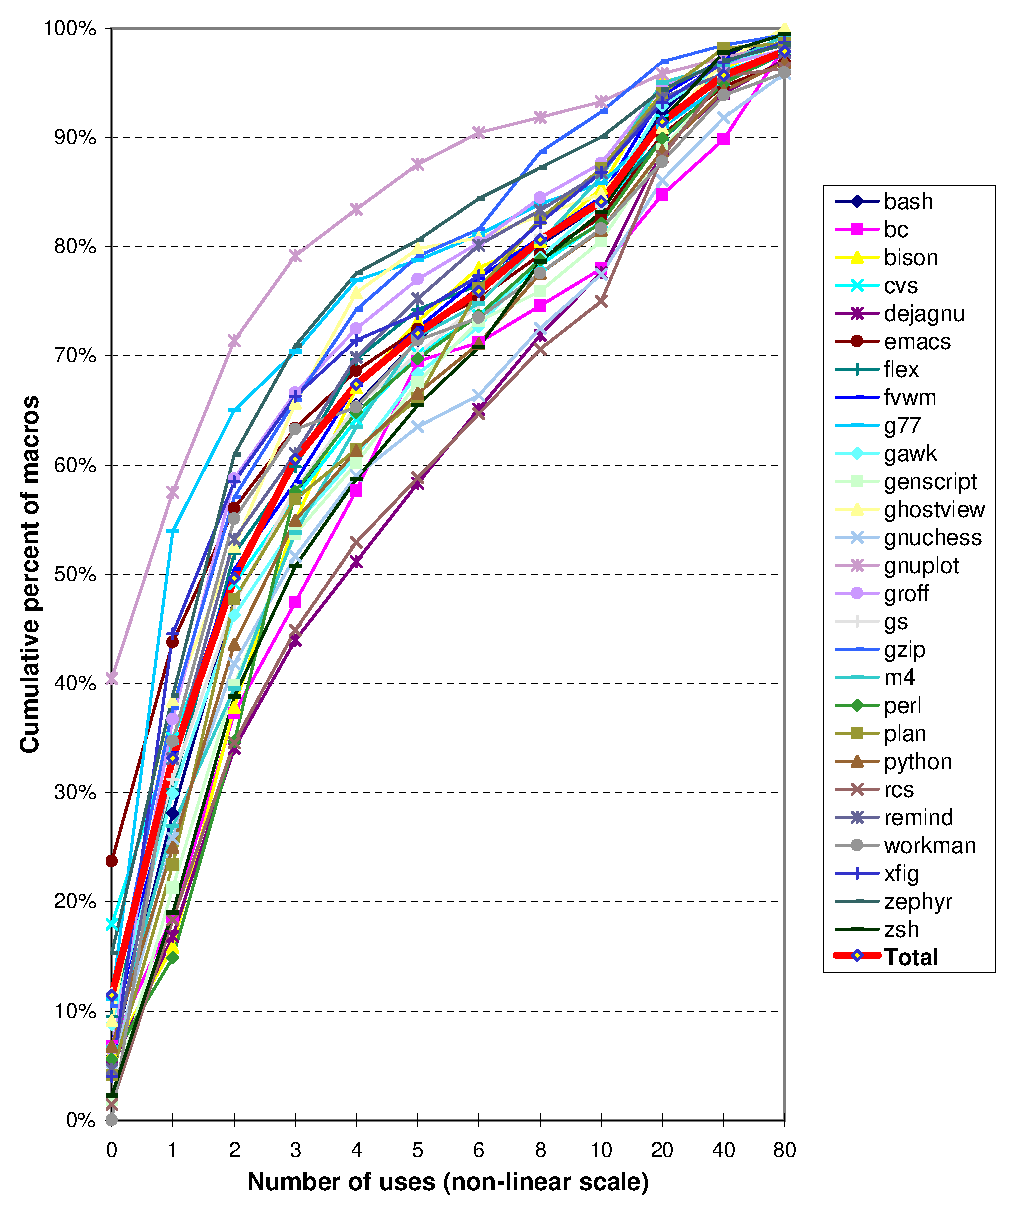
\epsfig{file=fig/use-frequency.eps,height=7.5in}}
% \caption{Number of expansions per Cpp macro.  The numbers in the
%   table represent the percentage of identifiers which are expanded a given
%   number of times or fewer.  For example, \pkg{g77} expands 65\% of its
%   macros two or fewer times.}
% \label{fig:freq-use}
% \end{figure}

\begin{figure}
\centerline{\epsfig{file=fig/cat-use-frequency.eps,height=7.5in}}
\caption{Number of expansions per Cpp macro.  The numbers in the
  table represent the percentage of identifiers which are expanded a given
  number of times or fewer.  For example, 50\% of all
  macros are expanded two or fewer times. Higher lines indicate less usage.}
\label{fig:freq-use-cat}
\end{figure}

%[[Double-check all these numbers!]]
%The tail of this distribution is quite long, indicating that some macros
%are used very heavily.  Ninety-nine percent of macros are expanded 147 or fewer
%times, 99.5\% of macros are expanded 273 or fewer times, 99.9\% are
%expanded 882 or fewer times, and \pkg{python} uses {\tt NULL} (which \pkg{python}
%itself defines) 4233 times.  Figure~\ref{fig:freq-use-cat} weights each macro
%equally rather than weighting each macro use equally, which would weight
%\pkg{python}'s {\tt NULL} 4233 times more heavily than a macro used only once
%and infinitely more than a macro never used at all).

\begin{figure}
  {\small\centerline{\begin{tabular}{|l|c|c|c|c|} \hline
 & \multicolumn{2}{c|}{one configuration}
 & \multicolumn{2}{c|}{all files} \\ \hline
 & & \multicolumn{1}{c|}{differing} & & \multicolumn{1}{c|}{differing} \\
 & \multicolumn{1}{c|}{defs} & \multicolumn{1}{c|}{defs}
 & \multicolumn{1}{c|}{defs} & \multicolumn{1}{c|}{defs} \\ \hline
Null define &            1.4 & 1.0 & 2.2 & 1.0 \\
Constant &               1.2 & 1.1 & 1.5 & 1.1 \\
Expression &             1.3 & 1.2 & 1.8 & 1.4 \\
Statement &              1.3 & 1.2 & 1.7 & 1.4 \\
Type &                   1.5 & 1.3 & 2.2 & 1.5 \\
Syntactic &              2.1 & 1.6 & 3.2 & 1.7 \\
Symbol &                 1.5 & 1.1 & 1.6 & 1.2 \\
Unknown symbol &         1.0 & 1.0 & 1.1 & 1.0 \\
Not C code &             1.4 & 1.4 & 3.9 & 2.7 \\
Failed classification &  1.7 & 1.5 & 5.9 & 3.7 \\ \hline
Total &                  1.2 & 1.1 & 1.8 & 1.3 \\ \hline
\end{tabular}


%%% Local Variables: 
%%% mode: latex
%%% TeX-master: "emp-use-2"
%%% End: 
}}
  
  \caption{Summary of
    figures~\ref{fig:freq-def-cat},~\ref{fig:freq-ddf-cat},
    and~\ref{fig:freq-use-cat}.  The table is by macro name.  Add percentages?
    [[The 1.0 distinct defs for unknown symbol is surprising; it indicates
    that it was the *same* unknown symbol in each definition (doesn't
    it?).  But a name is only in the category if none of its defs was
    recognized.  Double-check this!]]}
  \label{fig:freq-sum-cat}
\end{figure}

[[ Not sure what to say about figure~\ref{fig:freq-sum-cat}. --mernst]]
[[ I'd remove this figure, or use it without the uses column instead of
the distinct definitions figure. --gjb]]

\subsection{Macro usage in conditional control}

\begin{figure}
\centerline{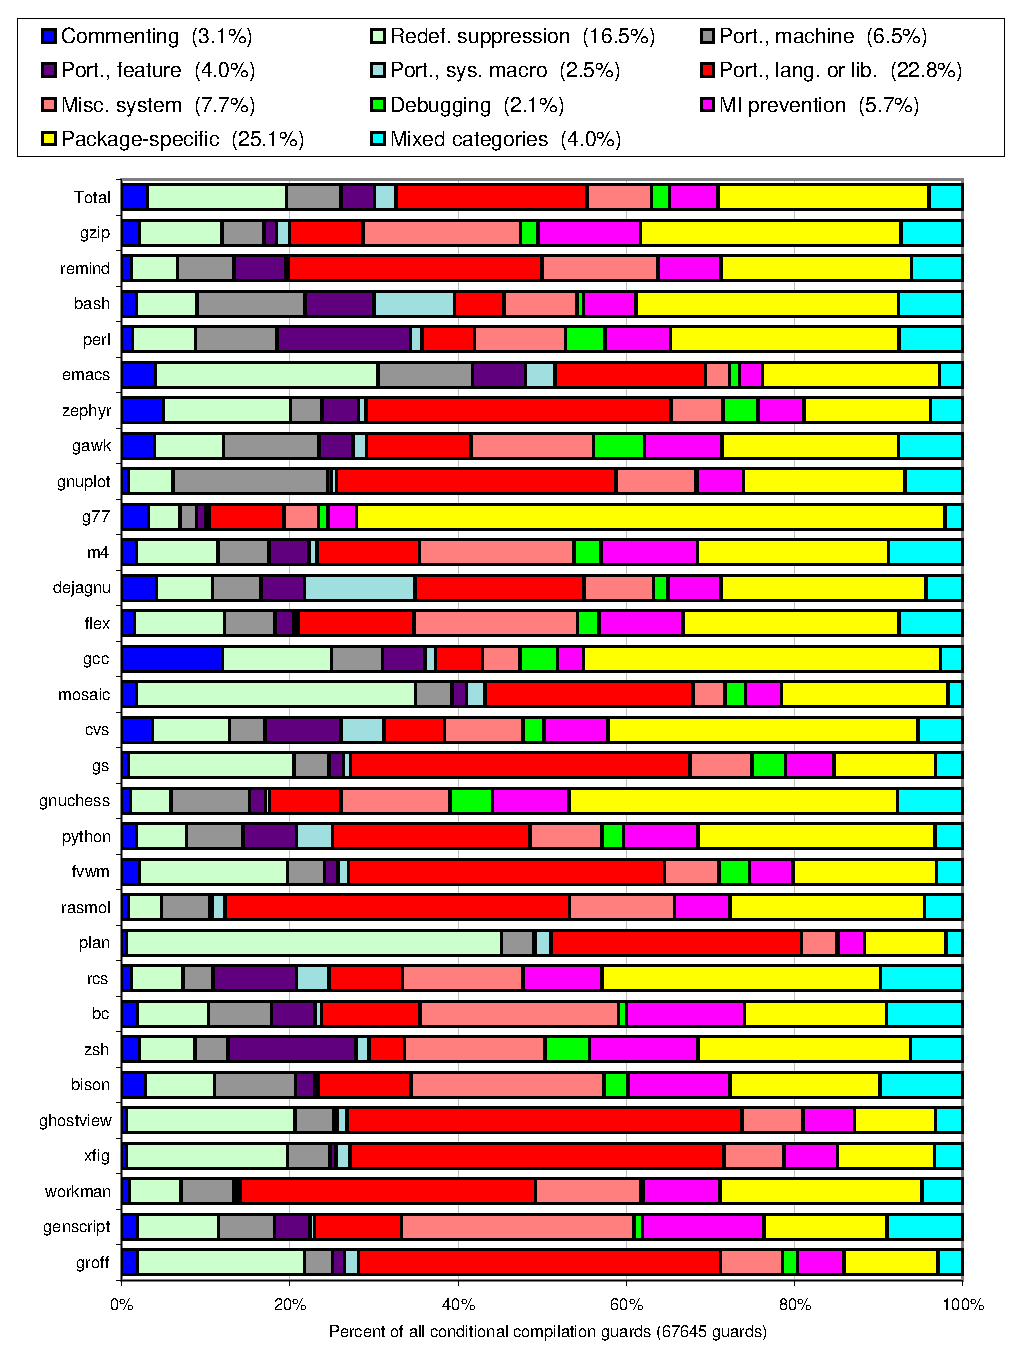
\epsfig{file=fig/ccd-categories.eps,height=7.5in}}
\caption{Categories for conditional compilation directives.}
\label{fig:ccd-categories}
\end{figure}

Conditionals are used to control inclusion of code for many different
reasons.  We categorized the uses of conditionals by the name and
context, and looked at how frequently conditionals are used for various
purposes.

{The following categories are based on macro names:

\begin{description}
%% See ccd_lexical_category in em_analyze for the routines
%% which implements these heuristics

\item[Package-specific] 
  These symbols are specific to the given package.  They do not fit any of
  the other categories.

\item[Portability, machine]
  These symbols name the operating system or machine
  hardware (e.g., \texttt{sun386} or \texttt{MACINTOSH}).
      
\item[Portability, feature]
  [[``feature'' is unhelpful; rename]] These symbols describe specific
  capabilities [[byte order isn't a ``capability'']] of the target machine
  or operating system (e.g., \texttt{BYTEORDER}, \verb|BROKEN_TIOCGWINSZ|).

\item[Portability, system macro]
  These symbols are commonly defined constants or
  pseudo-inline functions in system or language libraries (e.g.,
  \verb|O_CREATE|, \texttt{isalnum}, or \verb|S_IRWXUSR|).

\item[Portability, language or library]
  These symbols are predefined by a compiler, defined by a standard
  library, or defined by the package [[as part of the build
  process]] to indicate existence of compiler, language, or library features
  (e.g., \texttt{GNUC}, \texttt{STDC}, or \verb|HAS_BOOL|).

\item[Miscellaneous system]
  These symbols are reserved (i.e., they begin with two underscores) and do
  not fit any other category.
      
\item[Debugging]
  These symbols control inclusion of debugging or tracing code.  The macro
  names include \texttt{DEBUG} or \texttt{TRACE} (or both).
      
\item[Multiple inclusion prevention]
  These guards encompass an entire file to ensure that the enclosed code is
  seen only once per translation unit by the compiler.  Such guards are
  indicated by a trailing \verb|_H| or \verb|_INCLUDED| in the macro name
  they check.
\end{description}


These have to do with the entire guard, or with context:

\begin{description}
\item[Commenting] These guards either definitely succeed and
  have no effect as written (e.g., \texttt{\#ifdef 1}), or definitely fail
  and unconditionally skip a block (e.g., {\tt \#ifdef (0 \&\&
    \verb|OTHER_TEST|)}).  These guards are used to comment out code or to
  override other conditions (e.g., to unconditionally enable a previously
  experimental feature).
      
\item[Redefinition suppression] These guards test non-definedness of
  symbol, and control only  a definition of the same symbol, thus avoid preprocessor
      warnings about a redefinition of a name (e.g., \texttt{\#ifndef
      FOO} followed by \texttt{\#define FOO ...} and \texttt{\#endif}).
    
    The purpose is to provide a default value used unless another part of
    the system, or the compilation command, specifies another value.

\item[Mixed categories] These guards test multiple symbols
      which independently fall into different categories (e.g.,
      {\tt \#if defined(\verb|STDIO_H|) || \verb|SYSV_SIGNALS|}).

      [[Can ``mixed'' ever result from commenting or redefinition
      suppression?  Which has precedence, ``mixed'' or those?  (I hope
      those!)  So perhaps put these before the macro name heuristics.]]

\end{description}

%%% Local Variables: 
%%% mode: latex
%%% TeX-master: "emp-use-2"
%%% End: 
}

Figure~\ref{fig:ccd-categories} shows how each package uses macros in
conditional compilation directives.  There is significant variation
among packages, but overall portability is a major use of conditional
compilation directives.  Redefinition warning suppression, at 16.5\%, is
surprisingly high, and is essentially a macro definition mechanism, not
a conditional inclusion technique.  Encouragingly, mixed categories were
relatively rare; these correspond to conditional inclusions whose
meaning and intent is especially unclear.  Additionally, the low mixed
categories suggests that the conventions for macro names are fairly
standardized.

[[ The macros with mixed usage (especially here, but also in the
previous section) are akin to Krone \& Snelting's anomalous macros that
interfere in the lattice.  But we found more than they seemed to!  Did
we analyze the package in which they found their problem?  I'd like to
somehow be able to compare. --mernst]]
      

\subsection{Inconsistent usage}

Macros have two general purposes: they can control the inclusion of
lines of code (by appearing in a \texttt{\#if} condition that controls
that line) or can change the text of a line (by being expanded on that
line).  Each of these uses can correspond to language features---normal
\texttt{if} clauses or (for certain types of substitution) {\tt const}s
and {\tt inline}s.  But when a macro is used in both ways, something
more subtle is occurring, and there is
no easy mapping to a language feature.  It is harder to understand
and analyze a macro that is used in both ways.

We split macro uses into three categories:
\begin{itemize}
\item uses in C code, where the macro's expansion controls textual
      replacement; 
\item uses in \texttt{\#if}, \texttt{\#ifdef}, \texttt{\#ifndef},
      \texttt{\#elif} conditions;\footnote{We discarded uses in Cpp
        conditionals whose only purpose was to prevent redefinition.
        More specifically, if the condition tested only definedness, the
        next line defined the macro just tested, and the line after that
        ended the CPP conditional.  This is a bit overrestrictive, but
        conservative, and in practice quite accurate.} and
\item uses in the body of a macro definition.\footnote{These eventually
        bottoms out to one of the other contexts if that definition is
        ever used.  Uses in a macro body generally are intended to be
        used however the containing macro is.  Since those uses also
        appear in the figure, we did not attempt to track each such use
        in a body to some macro's appearance in either code or a
        conditional.}
\end{itemize}

%        A definition isn't a use of the macro being defined, only of those
%        in the body.  Since those are uses, 12\% is a lower bound on those
%        that never affect the code. It would be reasonable to assign the
%        5.4\% that are macro only, to the other categories on a pro rata basis.
%
%        Thus, the interesting categories are "code",
%        "conditional", "code and conditional", and "no use".

\noindent Figure~\ref{fig:where-used} reports on the ways that macro
names are used.  It shows that macros are expanded ten times more often
than they are used to control source code inclusion.  (However, each
inclusion use can control many lines of code; see
Section~\ref{sec:dependence}.)  The potentially subtle uses are those
for which a macro appears both in code and in a conditional.

Our data shows that packages use macros either to direct conditional
compilation or to produce code, but not for both purposes. This
separation of concerns makes the source code easier to understand.  Only
3.4\% of macros both expand in code and are used in conditional
contexts.\footnote{Plus a similar percentage of those used in other
  macro definition bodies, probably bringing the total up only another
  fraction of a percent to around 4\%.}  

%Conditional usage is rare in
%general; conditional compilation accounts for half of Cpp directives but
%only 7.1\% of macro usage (plus the categories just listed above).  But
%each use in a conditional can have a large effect on the system.


\begin{figure}
{\small
  \setlength{\tabcolsep}{.25em}
  \begin{tabular}{|l|r|}\hline
Code & 59.7%\\\hline
Code, macro & 11.4%\\\hline
Cond. & 6.4%\\\hline
Cond., macro & 0.3%\\\hline
Macro & 6.2%\\\hline
Code, cond. & 1.6%\\\hline
Code, cond., macro & 0.6%\\\hline
No uses & 13.9%\\\hline
Total & 22336 & (100%)\\\hline
\end{tabular}
%
}
\caption{Where macros are used: in C code, in macro definition bodies, in
  conditional tests, or in some combination thereof.  The numbers don't sum to
  100\% because of rounding.  [[It might be interesting to see this
  broken down by category.]]}
\label{fig:where-used}
\end{figure}



%[[Move this to the previous section, and reference back to it.]]
%      A surprising number -- nearly 12\% -- of macros defined in a package
%        are never used at all.  Occasionally [[find a concrete example of
%        this]] this is a result of shipping a 
%        standard set of headers with the package -- it's like a library for
%        that development team, but one that can't be counted upon to exist
%        everywhere, so it has to be provided.  For gnuplot, over 40\% of
%        macros are never used because the package's support for several
%        terminal types, such as tgif, is unfinished (and thus unused).
%        Even discounting that package, though, the numbers are remarkably
%        high.  We would be surprised if one in eight functions and
%        variables in a package were never used, not even in testing code.
%        [[Do we have any idea what fraction this is in practice?
%        Ask Dave Grove; he can compute this relatively easily.]]
%        (The percentage of macros defined in libraries/standard header
%        files which are never used in the code is enormous, but that is
%        expected.)

%      Across packages, there is heavy variation.  Packages which use
%        the preprocessor sparingly are as likely to have a high percentage
%        of mixed usage as packages which make heavy use of CPP.  (There is
%        a slight tendency for the less aggressive packages (i.e.,
%        those lower on the lists in figures~\ref{fig:directives-breakdown}
%        and~\ref{fig:categorization}) to have more uses in code, fewer uses
%        in conditionals, and fewer macros that are never used.)


\subsection{Number of arguments}

\begin{figure}
\centerline{\epsfig{file=fig/cat-numargs.eps,height=4in}}
\caption{Is this worth including?
  [[PROBLEM:  the numbers in this legend don't accord with those in
  previous legends by name.  This is because the numargs information was
  gleaned from the .catg file which contains only the macro bodies and
  the filename they were found in, thus there is no way to include macro
  bodies defined outside the package of macro names that are defined
  somewhere inside the package as is the case almost everywhere else;
  I'm now thinking that this information could've/should've been used
  for aiding the categorizations: i.e., a null define taking no
  arguments is a lot different than one taking arguments;  since that
  wasn't done, I'm inclined to drop this since to avoid the
  inconsistency in the numbers (and because it is of questionable
  utility as presented now --gjb]]}
\label{fig:cat-numargs}
\end{figure}


You might wonder whether macros are used like functions (taking arguments)
or like constants (taking no arguments).  
[[However, a fair number of statement macros also take no arguments.]]
We graphed that in
figure~\ref{fig:cat-numargs}.  This seems irrelevant to me; I don't see
where to fit it in, or what to say about it.



\section{Dependences}
\label{sec:dependence}
\label{sec:last-content-section}

[[Perhaps settle on a single name for each of the types of dependence, and
be consistent throughout (and in the figures).]]

Macros control the program which results from running Cpp in two
distinct ways.  {\em Inclusion} or {\em control} dependence results from
Cpp conditionals testing macros (for definedness, or by examining
expansions) to determine which which lines of the Cpp input appear in
the output.  {\em Substitution} or {\em expansion} dependence results
from replacement of macros outside Cpp conditionals by their definition
bodies, which controls the content of the lines on which the macros
appear. This section examines these dependences, breaking them down both
by macro and by line.

[[This is just a wretched description of the algorithm.  Fix?  Or is it
good enough?]]

%%% Old style LaTeX commands used below!

We computed, for each line, which macros it depends upon, and the variety
of dependence.  A line \emph{directly} depends on a macro that either
appears in the line or appears in a {\tt \#if} condition whose scope
contains the line.  A macros may also control a line indirectly, by
controlling the definition of another macro that controls the line.  For
instance, after {\tt \#define \verb|S_ISBLK|(m) ((m) \& \verb|S_IFBLK|)},
the final text of a line that uses \verb|S_ISBLK| depends not just on its
definition but also on that of \verb|S_IFBLK|.  These transitive
dependences are expansion dependences only if every direct dependence is an
expansion dependence; otherwise, the transitive dependence is an inclusion
dependence.

Our system does track dependences across file boundaries: if a macro
controls whether a file is {\tt \#include}d, then the macro also controls
every line of that file and anything controlled by macros defined in the
file.  We did not distinguish must from may dependences.  When there were
multiple different conditions that could lead to inclusion of a line, we
did not keep track of their boolean connectives, only of the individual
tests (like those appearing on a single {\tt \#if} line).  When
interactions among files are considered, these relationships may become
complex.

%% This makes absolutely no sense.  What is going on here?
%% I think there's something meaningful about lopping off prefixes of must
%% dependences, but can't puzzle it out now.  -MDE 11/1/97
% When different conditions control different definitions of a macro, uses
% are dependent on the independent parts of those conditions.  For instance,
% after
% \begin{verbatim}
%   #if A
%     #if B1
%       #define M ...
%     #elsif B2
%       #define M ...
%     #else
%       #define M ...
%     #endif
%   #endif
% \end{verbatim}
% a use of macro {\tt M} is expansion-dependent on {\tt B1} and {\tt B2}, but
% not on {\tt A}, which must have been set to true in order for {\tt M} to be
% defined at all.  That is, no setting of {\tt A} can affect {\tt M}'s


This section reports on only {\numpackageslesstwo} packages; it omits
Emacs and Mosaic, for which the space requirements for the full
dependence information exceeded our computer's virtual memory.  These
packages' excessive dependencies result in part from use of Motif, a
complex external library.  (We did generate complete dependence
information for Plan, which is the smallest of the three packages which
use the Motif library.)  Since two of the most aggressive users of
macros (and most highly dependent on macros) packages are omitted, the
numbers are smaller than might be expected in the presence of more
complete information.


\subsection{Dependences by line}

\begin{figure}
\centerline{\epsfig{file=fig/dep-byline.eps,height=4in}}

\caption{Percentage of lines dependent on a particular number of macros (or
  fewer).  For instance, 93\% of all lines are expansion-dependent on two
  or fewer macros, and 90\% of all lines are inclusion-dependent on 27 or
  fewer macros.  The log scale is shifted by unity in order to place 0
  on the scale; that is, we added 1 to each of the x axis values, before
  plotting, then relabeled ``1'' as ``0''.}
\label{fig:dep-byline}
\end{figure}

Figure~\ref{fig:dep-byline} graphs the percentage of lines dependent on a
given number of macros.  Over two in five lines (42\%) are controlled by
macros.  Most of these (38\% of all lines) are inclusion-controlled by at
least one macro; some of these lines, such as those in header files, may
always appear but be inside a guard to avoid multiple inclusion.  Over one
in four lines (28\%) expands a macro, which is higher than we had
anticipated.  

Multiple expansion dependence is not prevalent\,---\,only 5\% of lines are
expansion-dependent on more than 3 macros, and only 1\% are
expansion-dependent on more than 7 macros.  However, one line of
\pkg{gcc}\,---\,{\tt \verb|LEGITIMIZE_ADDRESS| (x, oldx, mode,
win);}\,---\,is expansion-dependent on 187 different macros.  Macro
\verb|LEGITIMIZE_ADDRESS| is defined 30 times in \pkg{gcc}, many of them
dozens of lines long and themselves studded with macro invocations.
However, only 13 lines in \pkg{gcc} are expansion-dependent on more than
100 macros.

Inclusion dependences have a much wider distribution.  One in twenty lines
is inclusion-dependent on at least 133 macros, and 1\% of lines are
dependent on over 300 macros.  As an example, the line of \pkg{gcc}
mentioned above has 187 inclusion dependences (more than its expansion
dependences, with only 13 macros in common between the sets), but over over
10,000 lines of \pkg{gcc} have even heavier inclusion dependences than
that.

On average, each line is expansion-dependent on .04 macros,
inclusion-dependent on .31 macros, and any-dependent on .34 macros.  (The
.01 macros that each line is, on average, both expansion- and
inclusion-dependent upon is included only once in the any-dependence
total.)

      

\subsection{Dependences by macro}

    We combined these charts for the different packages, because the shapes
      of each were quite similar for each package.  In order to permit
      combining charts across quite different package sizes, we computed
      values that were percentages of package size.

   \subsubsection{expansion}

\begin{figure}
% This works, but the figures are upside-down.
% \centerline{\epsfig{file=fig/exp-dep-bymacro.eps,angle=90,height=3.75in}}
% \centerline{\epsfig{file=fig/incl-dep-bymacro.eps,angle=90,height=3.75in}}
% Can't use ``height'' when rotating by -90 or +270; I don't know why.
\centerline{\epsfig{file=fig/exp-dep-bymacro.eps,angle=270,width=.85\linewidth}}
\bigskip
\centerline{\epsfig{file=fig/incl-dep-bymacro.eps,angle=270,width=.85\linewidth}}
\caption{Dependencies by macro name for 28 packages.
  Each bar represents all macros that control less than the labelled
  percent of the lines in its package (but more than the previous bar).
  For instance, the .17 bar in the expansion dependence chart on top
  indicates that there are 286 macros that each control between .11\%
  and .17\% of the entire package containing that macro.  The maximum
  falls in the last bucket specified (i.e., the first bucket off the
  chart is the first empty one).}

%% expansion is red; inclusion is blue
\label{fig:dep-bymacro}
\end{figure}

Practically every {\tt \#if} line (which accounts for about half of the
conditional compilation lines) expands a macro.  (Some don't, for instance
when testing which character set is being used on the compiling machine.)

        This exponential decay indicates that, as expected, there are more
          macros which control just a few lines and fewer macros that
          control a lot of lines.

        Outliers (> 6\% of all lines expand):
          int in gcc (14.85\% !)
          NULL, ANY, object in python

        Above 5\%: 
          SvANY in Perl
          const in RCS
          ip in workman -- bogus, as defined just twice, then undefined;
                  most places it is a formal parameter and out of the scope
                  of the macro definition.
          ArgCount, Args in xfig (like argc, argv)
          rtx in gcc (defined to int or int*)

        Overall, for these top 10:  6 types, 1 constant, 3 expressions

   \subsubsection{inclusion}

        For each package, the graph is bimodal (so much so that this even
          shows up a bit on the combined chart; it's more marked in the
          individual packages, I think).  Most macros control inclusion of
          no, or very few, lines; but quite a few control a substantial
          fraction of the package (around 10\%).

        All the heaviest dependences are on header files (for instance,
          \verb|H_PERL| controls inclusion of over 53\% of Perl's lines).

        [[It would have been interesting to run these numbers for everything
          but exclude file multiple inclusion prevention macros.]]


\subsection{CPPP experiment}

    [[After the above, this experiment doesn't sound like such a smart thing
      to try any more; its results certainly aren't unexpected.]]

    We had noticed in our programming that a particularly heavy use of the
      preprocessor is to handle multiple dialects of a language.  These uses
      tend to be less structured:  they don't have a simple pattern.  And
      this work must be done in the preprocessor:  there's no hope of
      integrating it into the language.  So we performed an experiment to
      see whether standardizing on a single language would reduce
      dependences, failed classifications, etc.

    We built a Cpp partial evaluator (called Cppp) which, given a set of
      macros known to be defined or undefined (and, optionally, their
      expansions), eliminates all possible Cpp conditionals.  We defined
      all the macros that can be depended on if using ANSI standard C or
      C++ (including prototypes and booleans) with POSIX-compliant
      libraries, preprocessed all the source (and 
      all library header files), and reran our experiments.

    The results were disappointing:  while some numeric measures of how
      complicated the resulting program's dependences are decreased, most
      remained at about their previous level.  The number of multiple
      definitions of macros, and the number of failed classifications, did
      not decrease as much as anticipated.

    From this we can conclude that there is no one obvious single point of
      attack:  even eliminating what seems most prevalent to us doesn't
      make a sufficient difference.



\section{Related work}
\label{sec:related}

Split this into:
 * taxonomies
 * checking tools
 * understanding tools such as Emacs hideif mode
 * other?

We could find no other empirical study of the use of the C
preprocessor nor any other macro processor.  However, we did find some
guidance on using C macros effectively and tools for checking macro
usage.

Carroll and Ellis state that ``almost all uses of macros can be eliminated
from C++ libraries''~[p.~146]{Carroll95}.  They list eight categories
of macro usage and explain how to convert them into C++ mechanisms.  They
do not discuss automatic conversion, but focus on instructing the software
engineer on better ways to do Cpp-like things.  Our work differs in at
least two ways.  First, our categories are somewhat different; we
believe that this is because ours were derived based on repeated
analyses of our data, rather than defined {\em a priori\/}.  Second,
we don't focus only on macros that could be converted to C++, since we
were interested as well in understanding which macros posed problems
to such as effort.

Similarly, a number of organizations provide hints about effective
ways to the use the C preprocessor.  The GNU documentation [[must
cite!  Is this the Cpp manual?  That should be cited somewhere
anyway]] discusses a set of techniques including simple macros,
argument macros, predefined macros, stringization macros,
concatenation macros, and undefining and redefining macros.  It also
identifies a set of ``pitfalls and subtleties of macros''; these are
much like some of the problems our analysis tool identifies.

We discovered that these categorizations sometimes focussed on constructs
that don't happen very often or missed ones that are actually frequent.
Our effort not only categorizes problems, but it also determines the
frequency of appearance of those problems and discovers other idiosyncratic
uses.

The Lint program will warn about empty statements, constants in conditional
context, and a few other things.  But it's pretty inadequate.  This mostly
has to do with problems after expansion.

A number of tools check whether specific C programs satisfy particular
constraints.  The lint program checker [[reference]]
checks for potentially problematic uses of C\@.  



Greg:  describe LCLint methodology and results.  Say exactly what you did
(i.e., how hard you tried), and what the results were.  Also, that you tried
on only 20, not all 30, packages, which doesn't include the biggest ones.


LCLint performs many of lint's checks and also
allows the programmer to add annotations which enable additional
checks~\cite{Evans-fse94}.
LCLint optionally checks function-like
macros\,---\,that is, those which take arguments\,---\,for
macro arguments on the left hand side of assignments, for statements
playing the role of expressions, and for consistent return types.
LCLint's approach is prescriptive: programmers are encouraged not to use
constructs that might be dangerous, or to change code that contains such
constructs.  We are more interested in analyzing, describing, and
automatically removing such uses so that tools can better process existing
code without requiring human interaction or producing misleading results.

LCLint
considers assignment to a macro argument dangerous but does not appear
to check for assignments to local variables.~\cite[\S 8]{Evans:LCLint}
[[Should we mention these things?  I don't want to seem nitpicky or petty, so
if we mention this, mention them as differences, not as things LCLint does
wrong.
\begin{quote}
$\ldots$ a parameter to a macro may not be used as the left hand side
of an assignment expression $\ldots$, a macro definition must be
syntactically equivalent to a statement $\ldots$ when it is invoked followed by
a semicolon $\ldots$, the type of the macro body must match the return
type of the corresponding function $\ldots$~\cite[\S 8]{Evans:LCLint}
\end{quote}
That quotation is really easy to nitpick:
\begin{enumerate}
 \item assignment parameters is fine (just turn into a reference argument) but
    assignment of non-parameters that aren't at global scope is quite bad.
 \item in x=foo(); we do NOT want foo() to be a statement
 \item a macro doesn't have a single type, but may have many polymorphic types
\end{enumerate}
]]


%% FIX: If we could also list the platforms for which each can compile,
%% that would be great, but I doubt the benefit is worth the effort for now

Krone and Snelting use mathematical concept analysis to determine the
conditional compilation structure of code~\cite{Krone94}.  They determine,
for each line, which preprocessor macros it depends upon, and display that
information in a lattice.  They do not determine how macros depend upon one
another directly, only by their nesting in {\tt \#if}, and the information
conveyed is about the program as a whole.  [[Compare to our CCD work, which
also tries to find such mismtches; and talk a bit more about what they
discovered and how it compares to what we discovered.]]


[[Expand; relocate in this section?]]
A limited number of tools do exist to assist software engineers to
understand code with containing Cpp directives, such as debuggers that can
call {\tt \#define}d functions and editors that support viewing one
particular configuration of the code.




\section{Conclusions}
\label{sec:conclusion}

[[Grist for conclusion: These data demonstrate that multiple definitions of
symbols is not numerically frequent; even more importantly, the definitions
of a symbol tend to be compatible, as shown in
section~\ref{sec:inconsistent}.]]


[[This is the place to recap the various sections, giving the highlights of
each.  (I think.)]]

% \subsection{Who cares?}
\subsection{Relevance of the results}

The results of this research are of interest to language designers, tool
writers, programmers, and software engineers.

Language designers can examine uses of the macro system's extra-linguistic
capabilities to determine what programmers consider missing from the
language.  Future language specifications can support (or prevent!)\ such
practices in a more disciplined, structured way.

% [[[Think more about this:  Also, how do language choices lead to more/less
% tightly integrated (as opposed to open, component-based) environments?
% E.G., no need for \verb|__LINE__| in Java?]]]

Programming tool writers, too, need to understand how Cpp is used, for that
sheds insight on the sorts of inputs that will be provided to the tool.  By
coping with the most common constructs, the tool can provide relatively
good coverage for low effort.  By identifying problematic uses, much better
feedback can be given to the programmer, who can be more effective as a
result.  The analysis results also indicate the difficulty of processing [[wc]]
preprocessor directives; before these analyses, we did not know whether the
task was so trivial as to be uninteresting, so difficult as to be not worth
attempting, or somewhere in between.

The analyses are of interest to programmers who wish to make their code
cleaner and more portable, and can help them to avoid constructs that cause
tools (such as test frameworks and program understanding tools)
to give incomplete or incorrect results.

% Also, learn weird new Cpp tricks!

Finally, our results are of interest to software engineers for all of the
above reasons and more.  Since this is the first Cpp usage study of which
we are aware, it is worth performing simply to determine whether the
results were predictable a priori; we did in fact discover a number of
interesting features of our suite of programs.


\subsection{Making C programs easier to understand}

The combination of C and Cpp makes a source text unnecessarily difficult to
understand.  A good first step is to eliminate Cpp uses where an equivalent
C or C++ construct exists, and to apply tools to explicate the remaining
uses.  Here we discuss a few approaches to solving this problem by
eliminating the source of confusion rather than applying tools.  We do not
seriously consider simply eliminating the preprocessor, for it provides
conveniences and functionality not present in the base language.

Since many of the most problematic uses of Cpp provide portability across
different language dialects or different operating environments,
standardization can obviate many such uses.  Canonicalizing library
function names and calling conventions makes conditional compilation less
necessary and incidentally makes all programs more portable, even those
which have not gone to special effort to achieve portability.  This
proposal moves the responsibility for portability (really, conformance to a
specification) from the application program into the library or operating
system, which is a reasonable design choice since many application programs
rely on a much smaller number of libraries and run on relatively few
operating systems.

Likewise, the most common single cause [[Really?  I'm not sure I believe
that without qualification]] for Cpp directives would be eliminated if the
C language and its dialects had only a single declaration syntax.  Because
most C compilers, and all C++ compilers, accept ANSI-style declarations,
much support for multiple declaration style may have outlived its
usefulness.  [[On the other hand, K\&R support was just *added* to some
mature, popular package (zsh?) recently.]]  We are investigating the effect
on our statistics (and program understandability) of ``partially
evaluating'' a program source by specifying the definedness and values of
some Cpp identifiers.

Some Cpp directives, such as {\tt \#include}, can be moved into the
language proper; this would also eliminate the need for Cpp constructs that
prevent multiple inclusion of header files.  Likewise, compilers that do a
good job of constant-folding and dead code elimination can encourage
programmers to use language constructs rather than relying on the
guarantees of an extra-linguistic tool like Cpp.\footnote{Interestingly,
  the issue seems to not be whether compilers do the appropriate
  optimizations, but whether programmers have confidence that the
  optimizations will be performed; if unsure, programmers will continue to
  resort to Cpp, since certainly a compiler cannot generate code for source
  that it does not ever even see (because Cpp has already stripped it
  away).}

Common Cpp constructs could be replaced by a special-purpose syntax.  For
instance, declarations or partial declarations could be made explicit
(perhaps first-class) objects; similar support could be provided for
repetitive constructs and dynamic scoping.  Manipulations of these objects
would then be performed through a clearly-specified interface rather than
via string and token concatenation, easing the understanding burden on the
programmer.  Such uses would also be visible to the compiler and could be
checked and reasonable error messages provided.  The downside of this
approach is the introduction of a new syntax or new library functions which
may not simplify the program text and which cannot cover all cases, only a
few specified ones.

[[Add a hygienic macros reference somewhere.]]

An alternative approach which avoids the clumsiness of a separate language
of limited expressiveness is to make the macro language more
powerful\,---\,perhaps even using the language itself via constructs
evaluated at compile time rather than run time.  (The macro systems of
Common Lisp and Scheme, and their descendants~\cite{WeiseC93}, take this
approach.)  An extreme example would be to provide a full-fledged
reflection capability.  Such an approach is highly general, powerful, and
theoretically clean; it circumvents many of the limitations of Cpp,
though it does not necessarily support all of Cpp's low-level features.
However, this approach may degrade rather than improve programs
understanding.  As difficult as it may be to determine what output a
macroless program produces, it can be just as difficult simply to determine
the text of a program which uses such macros.  (This is also a problem with
meta-object protocols, aspect-oriented programming, and intentional
programming, all of which permit the programmer to specify transformations
on other parts of the source code.  In practice, such systems are used in
fairly restricted ways, perhaps because other uses would be too
complicated.)  A dialog among users, compiler writers, tool writers, and
language theorists is necessary when introducing a feature in order to
prevent unforeseen consequences from turning it into a burden.


%% See slide 15 and its notes from Mike's quals talk.
\subsection{Future work}
 
These results suggest a wide variety of future avenues for research, both
in terms of expanding our understanding of uses of the preprocessor in
practice and in addressing the issues identified by this study.

[[Cut the repetition here.]]
In this work  we are concerned with how it {\em could} be used, not just how it {\em
  happens} to be used.  That's why we can't take the easy out.  But it
  would be interesting to look at uses, which would let us infer the {\em
  intended} use (if not all {\em possible} uses).  We are actively pursing
  this line of research.
A straightforward refinement that we are pursuing examines macro uses to
aid this categorization.  (For example, a macro used where a type should
appear can be inferred to expand to a type; a macro used before a function
body is probably expanding to a declarator.)
        We didn't examine every use.  Besides, the point isn't just the
          current uses, but also future uses:  we want these to be easy for
          programmers to use.

Further analysis of the conditional
compilation structure (in the style of Krone and Snelting~\cite{Krone94})
and of the macros with free variables (essentially achieving dynamic
scoping) is needed to see which of the roughly 29\% of expression macros
should be easy to convert to C++ language features such as constants or
enumerated values.
  [[We didn't analyze whether the free variables are globals or locals,
          which could substantially impact understanding/translation.]]


No libraries (e.g., \pkg{glibc}), as they're too different than applications.
No C++.\footnote{Preliminary results indicate that many
  C++ packages rely heavily on Cpp, even when C++ supports a nearly
  identical language construct, probably due to a combination of trivial
  translations from C to C++ and of C programmers becoming C++ programmers
  without changing their habits.}

``As with all benchmarks, there is the question of how representative this is.''
Variations among packages:
 * The C language has changed.  How do newer packages compare with older ones?
   [[Language changes are likely to make things worse, not better, in the
   short term, as code tries to compile under both while taking advantage
   of the new.]]
 * How do PC packages compare with Unix packages?  Less pressure to make it
   work on many platforms, because there aren't as many?
 * Correlate human perceptions of good or bad preprocessor use with what my
   tool says.
 * What's special about GNU programs?  Compare GNU to non-GNU?
 * Applications vs. libraries?  Get more libraries, or eliminate the current
   ones.




          
Reaching definitions for macros (``flow-sensitive'' due to
dependences on other macros).

Rather than storing information about a macro name, it's better to
recompute it (memoizing, perhaps) for each use so that I only refer to the
potentially applicable definitions (based on current must inclusion) -- but
still computing the must inclusion, expansion, and may inclusion from the
potentially relevant definitions.  



% Not really right:  Don't want the ``References'' section head to be small.
{\small \bibliography{evil}}

\end{document}
